\documentclass[a4]{MScthesis}
\usepackage{parskip}
\setlength{\parindent}{0cm}
\usepackage{ae}
\usepackage{pdfpages}
\usepackage{booktabs}
\usepackage{varioref}
\usepackage{natbib}
\usepackage{siunitx}
\usepackage{hyperref}
\usepackage{todonotes}



\title{Camera-assisted ROV navigation in sea cages} % The title of your assignement; NB use \newlinetitle to start a newline
\author{Morten Engelhardt Olsen} % Your firstname and lastname
\professor{Jo Arve Alfredsen, ITK} % Affiliation = ITEM for instance
\supervisor{Jo Arve Alfredsen, ITK\\ & Per Rundtop, SINTEF Fiskeri og Havbruk}

%% Uncomment the following in case you want subfigures; note that there will be a warning for the caption package
% \let\subcaption\undefined
% \let\subfloat\undefined
% \usepackage[bf]{caption}
% \usepackage{subcaption}

\DeclareGraphicsExtensions{.pdf,.jpg,.png}
\graphicspath{{./figs/}}

%\loadglsentries{glossary}
%\makeglossaries

\begin{document}
\selectlanguage{english}
\pagenumbering{roman}
\pagestyle{plain}

%% Only for the project
\titleITEM

\cleardoublepage
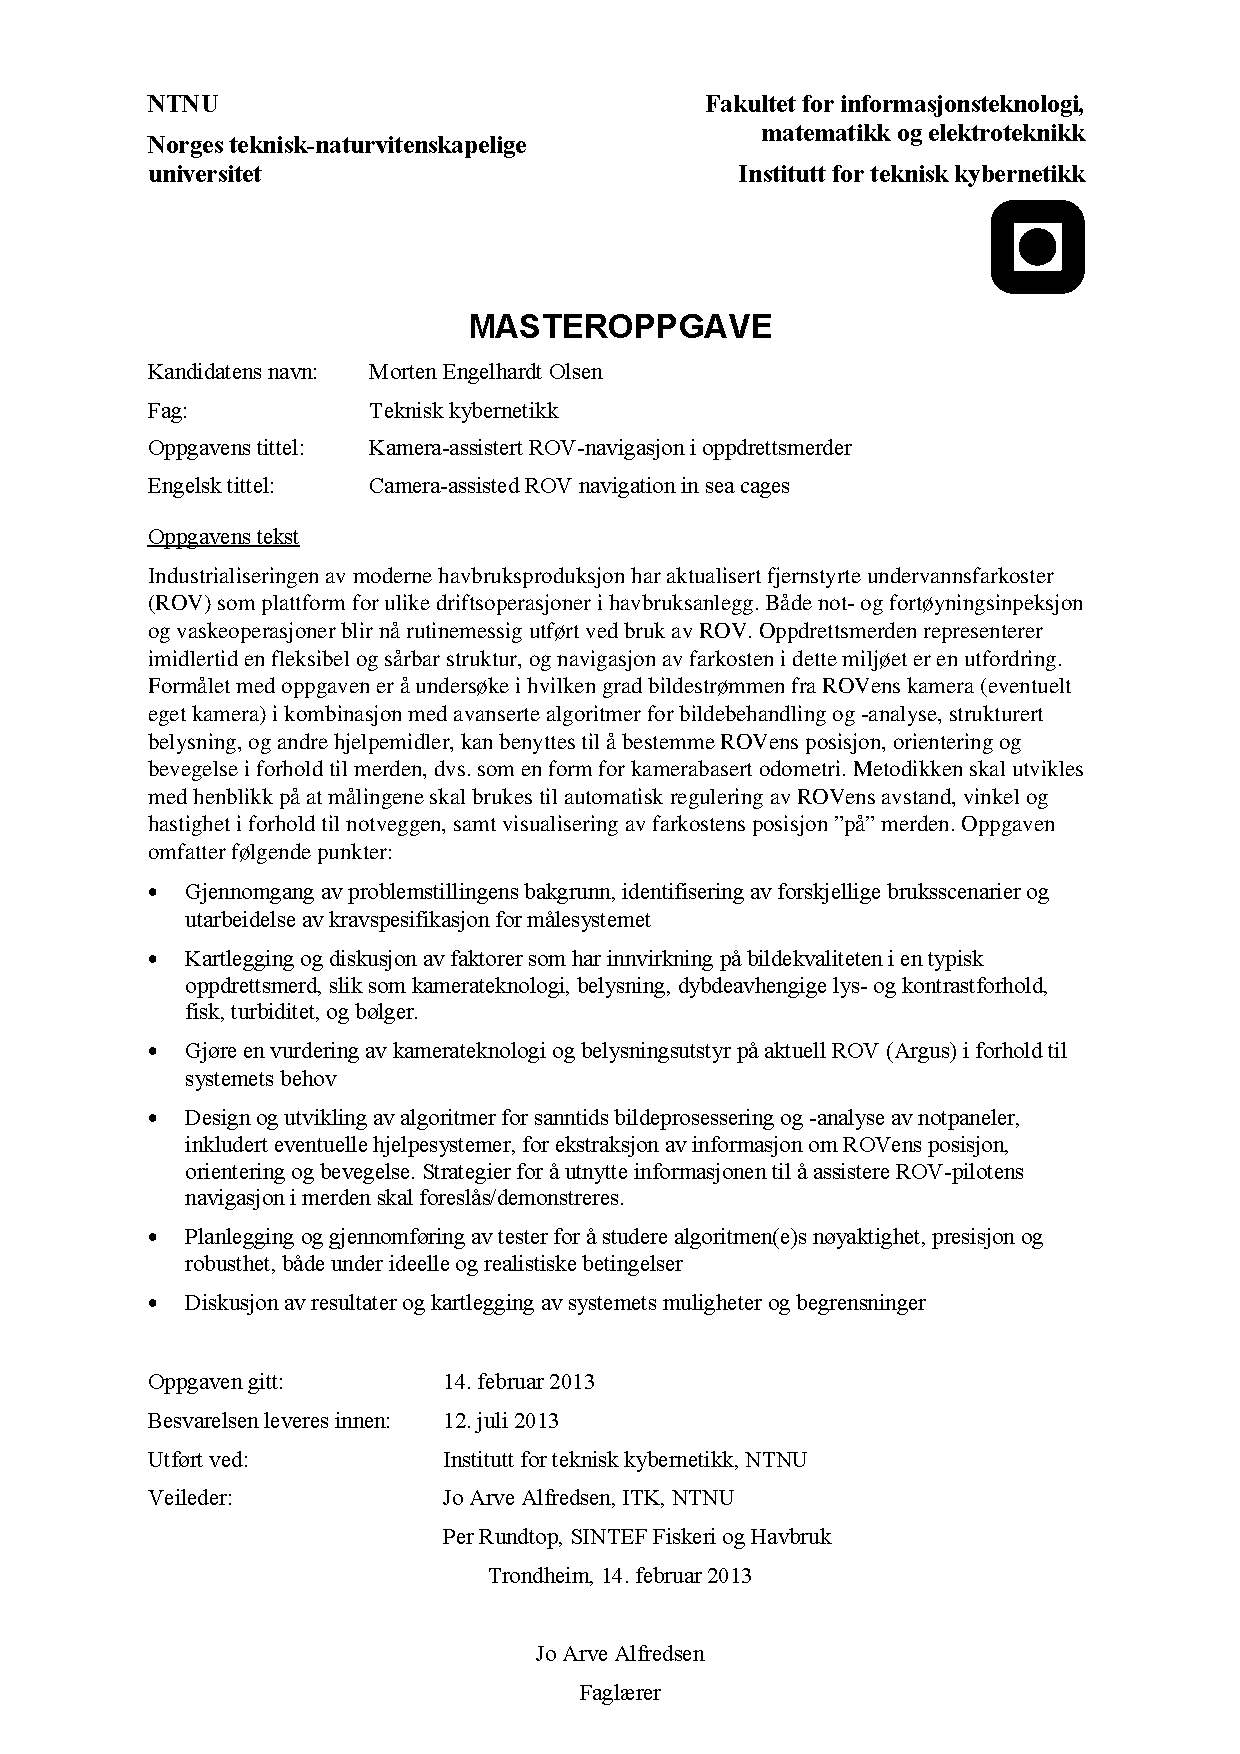
\includepdf[pages={1}]{assig.pdf}

%% Only for the master's thesis; for the project report the description is taken from It's Learning and added by the department
% \selectlanguage{english} % Change to 'norsk' if you are writing in Norwegian
% \input{problem_description}
% \cleardoublepage

%% There must be an abstract in English, even though the main text is in Norwegian
\selectlanguage{english}
\begin{abstract}
This thesis is a preliminary study of the feasibility of using 
modern computer vision algorithms for navigation in specific 
and known underwater environments. Using new high definition camera 
technologies and .... \todo{MORE}
\end{abstract}
\cleardoublepage

%% Only for the master's thesis; if the main text is in English and you can write Norwegian, there must be an abstract in Norwegian as well.A
% \selectlanguage{norsk}
% \begin{abstract}

\end{abstract}
% \cleardoublepage

\selectlanguage{english}% Change to 'norsk' if you are writing in Norwegian

%
\chapter{Preface}


\section{Acknowledgements}

I would like to thank Terje Haugen (ITK) at the departments mechanical workshop for 
helping with design and the actual making of the underwater housing for the test system.

A thank also goes to Kevin Frank (SINTEF) and Per Rundtop (SINTEF) for expertise 
in aquaculture and use of their test rig and cooperation in the field testing. 

A special thanks goes to Trond Viggo Melum (NRK) for help with troubleshooting the HD-SDI interface.

Thanks to Rolf Hansen (Malvik småbåtforening) for lending some space in the harbour for the rigging.

And last but not least, a big thank to Jo Arve Alfredsen (ITK) for support and 
brilliant guidance during the rougher times of this thesis.
\cleardoublepage

% similarly you may add a separate acknowledgments page

\tableofcontents*
\cleardoublepage

%% include if relevant
\listoffigures
\cleardoublepage

%% include if relevant
\listoftables
\cleardoublepage

%% include if relevant
%\listofalgorithms
%\addcontentsline{toc}{chapter}{List of Algorithms}
%\cleardoublepage

%% include if relevant
%\printglossary[title=List of Symbols, style=long]
%\cleardoublepage
%\glsaddall[]

%% include if relevant
%\printglossary[title=List of Acronyms,type=\acronymtype] % prints just the list of acronyms
%\cleardoublepage

\pagenumbering{arabic}
\pagestyle{ruled}



\chapter{Preface}


\section{Acknowledgements}

I would like to thank Terje Haugen (ITK) at the departments mechanical workshop for 
helping with design and the actual making of the underwater housing for the test system.

A thank also goes to Kevin Frank (SINTEF) and Per Rundtop (SINTEF) for expertise 
in aquaculture and use of their test rig and cooperation in the field testing. 

A special thanks goes to Trond Viggo Melum (NRK) for help with troubleshooting the HD-SDI interface.

Thanks to Rolf Hansen (Malvik småbåtforening) for lending some space in the harbour for the rigging.

And last but not least, a big thank to Jo Arve Alfredsen (ITK) for support and 
brilliant guidance during the rougher times of this thesis.
\cleardoublepage{}


\chapter{Introduction}
During the last four decades, the demand for fish 
has been steadily increasing. The current level 
of demand supersedes the amount of fish that 
can be fished and keep the different stocks of 
fish at a sustainable level. This has lead to 
overfishing, eliminating for instance the 
fish population on the Grand Banks off the east 
coast of America. Many other fish 
populations are also either gone or in fast 
diminish. Some scientists are even predicting 
that with the current overfishing, the fish industry will 
see a global collapse during this century \citet{worm06}.


\section{Motivation}


\section{Previous Work}


\section{Outline}


\cleardoublepage{}


\chapter{Specifications}
The hardware and software used in this project was chosen to be as close as possible to the 
hardware used by Argus in their underwater vehicles. This gives us 
a scenario closer to the real hardware, and imposes the same 
restrictions on us as would be imposed in real world applications.

This chapter goes through the main specifications of the hardware, its consistency with 
regards to what is available on ROVs, and comparisons where different techniques are available.
A introduction is also made to the software platform that were chosen, and some of the considerations 
regarding that choice.

\section{Hardware}

\subsection{Argus hardware}\label{sec:argus_hw}
The hardware used by Argus is only mentioned as 

\begin{itemize}
	\item $1\times$ Foc/Zoom camera
	\item Optional HDTV Camera 1080i
	\item $1\times$ Lowlight Black \& White camera
\end{itemize}

in \citet{argusROV}. After some mailing with Argus, they provided us 
with the specific details of this HD Camera, which is what we are interested in. 
The most interesting parts of the camera specification is shown in table \vref{tbl:fcbh11}.

\subsection{High definition video hardware}\label{sec:fcb_h11_hw}
The camera used by Argus is the Sony FCB-H11 \citet{fcbh11}. 

\begin{table}[htbp]
	\centering
	\begin{tabular}{ll}
	
		\toprule
			Camera specification 	& Detail \\
		\midrule
			Image sensor 			& 1/3-type CMOS \\
			Pixels 					& $\approx2\times10^{6}$ Pixels \\
			Zoom 					& $12\times$ (Digital) and $10\times$ (Optical) \\
			Gain 					& Auto and manual (\SI{-3}{\deci\bel} to \SI{18}{\deci\bel}) \\
			S/N						& > 50dB \\
			Minimum illumination 	& \SI{1.2}{\lux} (F1.8 50IRE) \\
									& \SI{1.0}{\lux} (ICR ON F1.8 50IRE) \\
			Video output			& HD Analog component Y/Pb/Pr \\
									& HD Digital LVDS Y/Pb/Pr 8 bit \\
									& SD VBS \SI{1.0}{\volt_{p-p}} Negative sync Y/C \\
			Camera control interface& VISCA TTL \\
			Operating temperature	& \SI{0}{\celsius} to \SI{45}{\celsius} \\
			Power consumption		& \SI{9}{\volt} $\pm$ \SI{3}{\volt} DC, \SI{4.8}{\watt} \\
		\bottomrule
	\end{tabular}
	\caption{Selected FCB-H11 Specifications}
	\label{tbl:fcbh11}
\end{table}


As seen in \vref{tbl:fcbh11}, the camera outputs HD Digital LVDS\footnote{Low-Voltage Differential Signal} signals.
Due to the open standard used by this camera, there are quite a few different add-on cards that 
converts this LVDS signal to other, more robust signals for different applications.

\subsubsection{VISCA camera control}\label{sec:visca}
The FCB-H11 can be controlled by the open Sony VISCA protocol. This is based of RS-232C at TTL signal levels
at 9600 bauds. Newer cameras can support RS-232C at up to 38400 bauds using a 8N1 configuration and no flow control. 
VISCA contains a rich set of commands to control professional video systems. It is even compatible with 
the broadcast networking specification of the RS-232C which means that a single signal line can contain 
8 devices including the PC, as it uses \SI{1}{\byte} for addressing.

The implementation of the VISCA protocol that is supported by the FCB-H11 is given in \citet{fcbh11tech}. 
The FCB-H11 does for instance not implement the broadcasting function of VISCA, and must therefore 
be on a single RS-232C signal line. 

In addition to normal power on/off and setup data, the VISCA protocol can send a slew of different 
control messages. Amongst these are zoom, focus, white balancing, spot focus and different video effects as 
black and white or negative images that is being processed by the image processor on the camera. This 
makes the camera very versatile, either by direct control from a PC using a TTL level translator or 
by any micro controller using USART.

Sony provides a basic program for testing and driving equipment through VISCA. In addition to this, a open source C library for Windows, Linux and 
AVR called libVISCA\footnote{Available at \url{http://sourceforge.net/projects/libvisca/}} has been developed. This makes it very easy to 
integrate VISCA into the software if needed as either a component or as a separate library. This also gives any software the 
possibility to control the camera to tweak the image stream.

\begin{figure}[htbp]
	\centering
	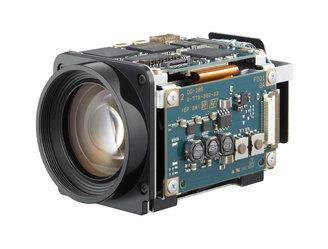
\includegraphics{fcbh11}
	\caption{Sony FCB-H11 High Definition Block Camera}
	\label{fig:fcb-h11}
\end{figure}

\subsection{High definition video signalling}

Many different interface boards are available for the FCB-H11 which gives different output formats from the camera and 
provides different control interfaces to the camera..
The most normal interface cards provides HDMI, USB, Ethernet, SDI and HD-SDI outputs in 
different configurations and combinations. A comparison of the different technologies is shown in \vref{tbl:transmission_systems}.

\begin{table}[htbp]
	\centering
	\begin{tabular}{llllr}
		\toprule
			System 				& Bitrate 							& Distance 						& Protocol 		& Compression Ratio \\
								& 									& 								& 				& (for 720p Video) \\
		\midrule
			HDMI 				& \SI{10.2}{\giga bit\per\second}	& $\approx$ \SI{15}{\metre}		& TMDS 			& 0\% \\
			USB 3.0 			& \SI{5}{\giga bit\per\second}		& $\approx$ \SI{5}{\metre}		& Serial		& 0\% \\
			Gigabit Ethernet	& \SI{1}{\giga bit\per\second}		& $\approx$ \SI{220}{\metre}	& Serial		& $\approx$ 30\% \\
			SDI					& \SI{360}{\mega bit\per\second}	& $\approx$ \SI{300}{\metre}	& NRZI 			& $\approx$ 75\% \\
			HD-SDI				& \SI{1.485}{\giga bit\per\second}	& $\approx$ \SI{300}{\metre}	& NRZI			& 0\% \\
			HD-SDI (optical)	& \SI{1.485}{\giga bit\per\second}	& $\approx$ \SI{45}{\kilo\metre}& NRZI (optical)& 0\% \\
			Dual Link HD-SDI	& \SI{2.970}{\giga bit\per\second}	& $\approx$ \SI{300}{\metre}	& NRZI			& 0\% \\
			3G-SDI				& \SI{2.970}{\giga bit\per\second}	& $\approx$ \SI{300}{\metre}	& NRZI			& 0\% \\
			6G-SDI				& Undecided\tablefootnote{Still in draft}& $\approx$ \SI{300}{\metre}& NRZI			& 0\% \\
		\bottomrule	
	\end{tabular}
	\caption{Different signalling and transmission systems available for video streaming.}
	\label{tbl:transmission_systems}
\end{table}


For this project, it was decided that we should 
try to get a interface that did have more capacity than the camera produces. Looking 
at the different options in \vref{tbl:transmission_systems}, the system from Argus and also thinking of the transmission length, HD-SDI
was chosen as the desired technology for transferring the video stream from the camera.

\subsubsection{HD-SDI}\label{sec:hdsdi}
The HD-SDI signalling standard is a improvement to the older SDI standard. Where the SDI can only transfer images
in maximum 576i format, the HD-SDI standard i capable of transferring 720p and 1080i video. Newer versions 
of the HD-SDI standard is also capable of 1080p and 4K video streams. 

HD-SDI is a professional video standard mainly used by TV stations and in other high end systems. It is 
defined and maintained by the Society of Motion Picture \& Television Engineers, SMPTE. More information 
on the SDI family can be found on the SMPTE website at \url{https://www.smpte.org/standards/}.

Some of the niceties of the HD-SDI interface, in addition to the bandwidth and transmission length, is 
that the interface is self-clocked, self-correcting and supports self-setup and initialization. This means that the 
interface is more or less plug-and-play. 

\begin{figure}[htbp]
	\centering
	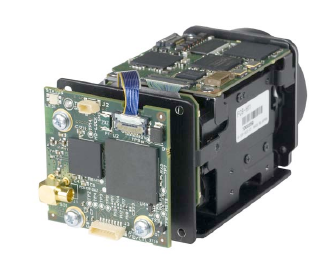
\includegraphics[width=0.8\linewidth]{em15710}
	\caption{Intertest EM15710 iShoot-FCB-HDSDI interface}
	\label{fig:em15710}
\end{figure}

This interface is coincidentally the same interface used by Argus according to the information that were received from them.
However, due to the long distance of transmission when a ROV is submerged, Argus does a on-board conversion of the 
coaxial HD-SDI signal to a optical carrier. The use of a optical medium to transfer HD-SDI is a normal 
technique when the high definition signals are transferred over a distance that would lead to signal degradation using 
electrical signalling.

The HD-SDI interface has also been extended into Dual Link HD-SDI, 3G-SDI and 6G-SDI. The Dual Link 
is a simple extension allowing two HD-SDI streams on one cable. The 3G version specifies a new signalling standard 
without changing the bitrate relative to the Dual Link. However, the 3G version is has full 
capability of 1080p streams at \SI{60}{\hertz}. Finally, the 6G version is a new and upcoming version made 
specifically for the new 4K, also known as Ultra HD, video format. The differences between the different resolutions can be 
seen in figure \ref{fig:resolutions}.

\begin{figure}[htbp]
	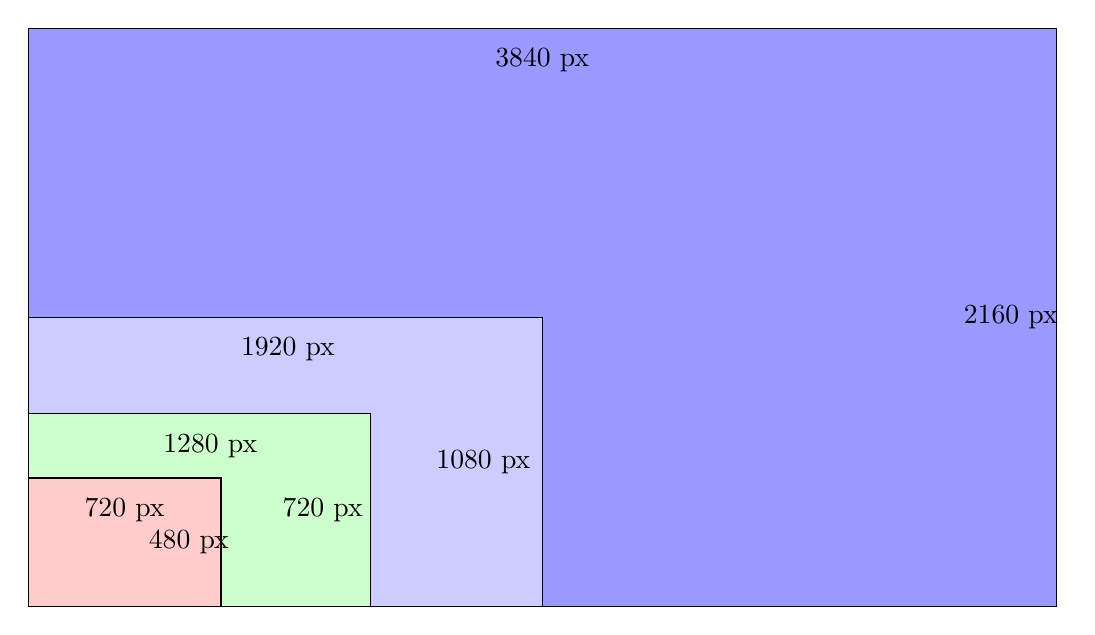
\begin{tikzpicture}[scale=0.34]
		\filldraw[fill=blue!40!white] (0,0) rectangle (38.4,21.6);
		\filldraw[fill=blue!20!white] (0,0) rectangle (19.2,10.8);
		\filldraw[fill=green!20!white] (0,0) rectangle (12.8,7.2);
		\filldraw[fill=red!20!white] (0,0) rectangle (7.2,4.80);
		
		\node() at (3.6,3.6){720 px};
		\node() at (6,2.4){480 px};
		
		\node() at (6.8,6){1280 px};
		\node() at (11,3.6){720 px};
		
		\node() at (9.7,9.6){1920 px};
		\node() at (17,5.4){1080 px};
		
		\node() at (19.2,20.4){3840 px};
		\node() at (36.7,10.8){2160 px};
	\end{tikzpicture}
	\caption{Scales of different resolutions. Red: DVD, Green: 720p, Light Blue: 1080p, Blue: UHD (4K).}
	\label{fig:resolutions}
\end{figure}



\subsubsection{Gigabit Ethernet}\label{sec:hw.gige}
During the last month of the project, two Gigabit Ethernet modules were acquired. The modules is primarily 
going to be used in future projects, as cabling and instrumentation over ethernet turns out to be simpler. 

The interface is shown in figure \vref{fig:iport} with the FCB-H11 connected. This unit gives access to the VISCA protocol described 
in \vref{sec:visca} over ethernet, together with the video feed. This means that the feed and control signals can be superimposed 
on any ethernet compatible infrastructure, which is both cheaper and more readily available, as well as easier 
to interface with most computers today.

\begin{figure}[htbp]
	\centering
	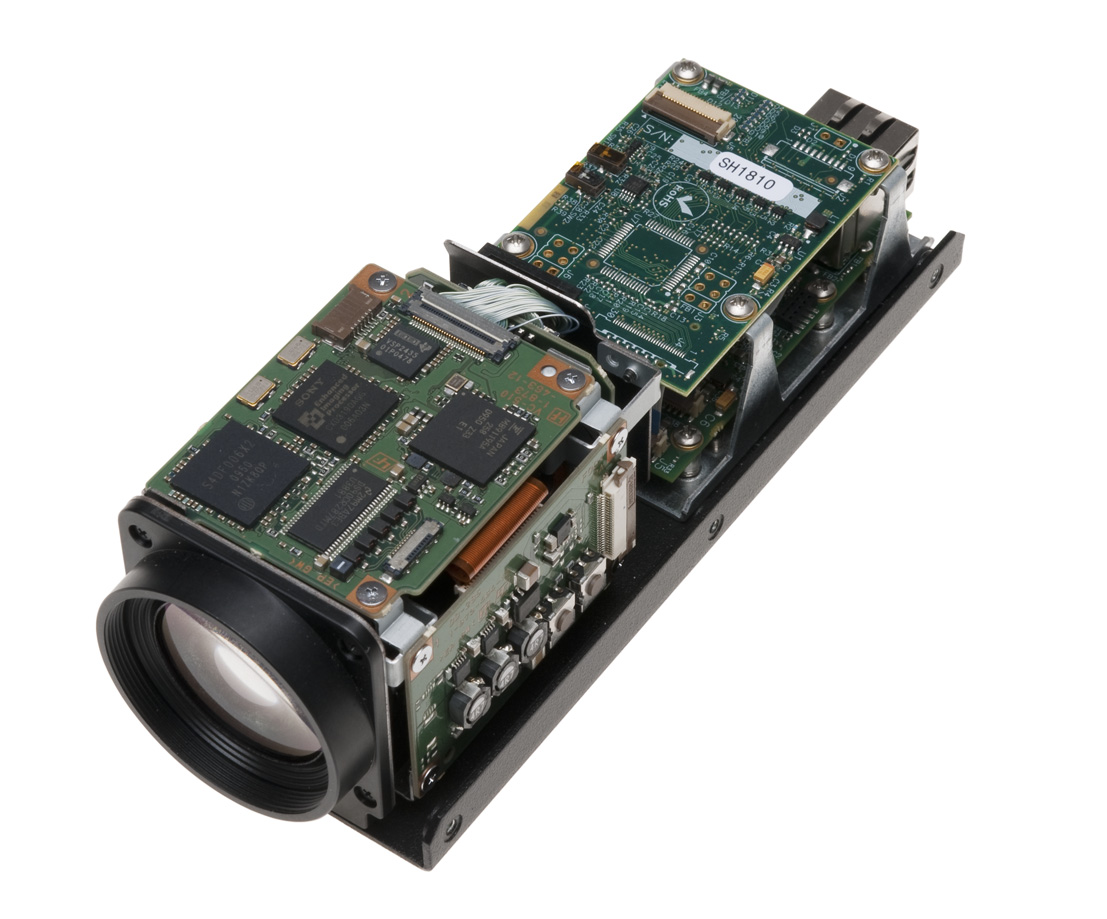
\includegraphics[width=0.8\linewidth]{iport}
	\caption{Pleora SB-Pro IP Engine for Sony FCB-H11}
	\label{fig:iport}
\end{figure}

\subsubsection{Video stream grabbing}
The capture of video streams from a HD-SDI interface usually needs specifically designed hardware that 
connects to one of the internal buses in the computer to get high enough bandwidth. This is usually 
done using a PCI Express card that can support multiple HD-SDI streams simultaneously. 

This is however not practical, as we are going to use different computers and laptops during our testing. 
It would therefore be better to get a external capture interface that connects to the computers using a 
external computer interface. Thankfully, with the development of USB 3.0 we are able 
to support the bandwidth requirements for HD signal, as the USB 3.0 has a theoretical maximum bitrate 
at \SI{5}{\giga bit\per\second}.

The Ultrastudio SDI from Blackmagic Design was chosen as the stream grabber. This is a industry standard 
supplier that recently developed this external capture unit. More information on this can be found at 
\url{http://www.blackmagicdesign.com/products/ultrastudiousb3/} and the unit is shown in \vref{fig:ultrastudio_sdi}.

\begin{figure}[htbp]
	\centering
	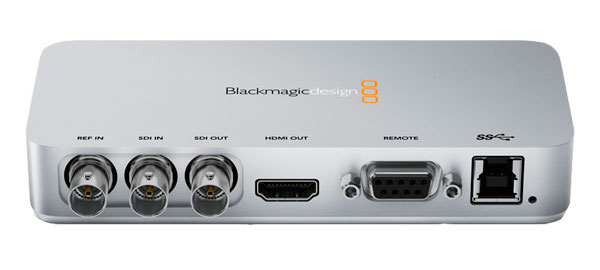
\includegraphics[width=0.8\linewidth]{ultrastudiosdi}
	\caption{Blackmagic Ultrastudio SDI for USB 3.0}
	\label{fig:ultrastudio_sdi}
\end{figure}

The Ultrastudio SDI unit gives HD-SDI in together with HD-SDI out, HDMI out and USB 3.0. The 
extra HDMI out makes it easy to connect a external monitor while capturing to get better visual feedback.

The ethernet module described in \autoref{sec:hw.gige}.uses multicast technology to transfer the video stream over IP. The 
card comes with a open SDK to discover and stream from any unit on the local network. As a added bonus, the 
ethernet module allows the VISCA control commands from section \vref{sec:visca} to be transferred over the same 
ethernet connection, removing the need for extra signalling cabling.

\section{Software}
The software used is split into two different categories; the video capture software provided by Blackmagic 
Design or any other compatible platforms, and the video analysis software developed in this project. Fortunately, the Ultrastudio 
unit comes with WDM\footnote{Windows Device Management} drivers and DSHOW\footnote{Direct Show, part of DirectX} 
filters, and a software development kit which makes it somewhat easy to connect to the unit and stream 
the video from it in real time. 

\subsection{High definition video capture}
In theory, all WDM compatible software can be used to access the video stream from the Ultrastudio unit. It turns out
however that the provided software from Blackmagic has some extra interfaces which makes it a bit easier to use, for instance 
to change resolution on demand, jitter removal and different behavioural aspects.

Blackmagic provides the Media Express platform for capture. This is a basic but useful starting point. The main 
drawback is the small amount of capture formats available in the software, and the frequent crashes that were experienced 
during use. However, the program were stable during capture, and it is capable to capture to YUV-8 bit which means almost 
as raw data as possible. This format is also easy to re-encode to other formats at a later stage for storage. 

It turned out that the image processing stack used in the project also were capable to connect directly to the Ultrastudio unit. 
This meant that the video stream could be fed straight into the different algorithms. This were useful for 
testing on-line performance, as opposed to storing the stream and doing off-line analysis.

\subsection{High definition video analysis}
The de facto standard in computer vision is the OpenCV library. Based on C++, it contains bindings multiple other languages. Especially 
the Python binding makes quick prototyping easy. Matlab was also considered, as Matlab does contain quite a powerful 
computer vision toolbox\footnote{Equivalent to library}.

During early prototyping, several discrepancies between the OpenCV algorithms 
 and the equivalent Matlab 
algorithms were discovered. Multiple standard algorithms would behave differently with the same source and same parameters. This 
were the cause of the shift from using Matlab as prototype platform to using Python as Python uses the same library source 
as the one used in C++.

\subsection{Real time considerations}


\cleardoublepage{}


\chapter{Computer Vision and Algorithms}

Computer vision has seen a substantial growth over the last 40 years, as camera technology became mature 
and the analysis of data became cheaper and faster. In this chapter we are going to look at the main algorithms 
that were tested and applied in the project, and give some more depth in the algorithms and mathematics behind each of them.

\section{Smoothing}\label{sec:smooth}\todo{MER!!!}
Smoothing is a normal technique in computer vision to remove artefacts and noise from images. The normal way 
of smoothing a image is to apply a filter to each pixel of the image through convolution. This makes 
all filter knowledge from the field of signal processing available.

The use of convolution also standardizes the structure of filters, and makes them easy interchangeable. Some 
of the most used filter kernels are shown in the following sections.

\subsection{Normalized Box Filter}\label{sec:box.filter}
The box filter with normalization is the simplest of all filters. Each pixel is convolved with a kernel 
that weights all neighbouring pixels equally.

\subsection{Gaussian Filter}\label{sec:gaussian.filter}
This is the most used filter. The kernel used in this filter approximates a Gaussian function. This kernel 
is usually generated based on a set size with given mean and variance which is then normalized.

\subsection{Median Filter}\label{sec:median.filter}
This filter is almost as easy as the Normalized Box filter in section \vref{sec:box.filter}. The only difference is that 
in stead of a normalized identity kernel, this kernel is the median of the pixel values of the neighbourhood.

\section{Hough Algorithms}
The set of Hough algorithms uses a trick to find lines in a image. The trick is 
instead of using the Cartesian description $y(x)=ax+b$ for lines, to rather use the 
a polar parametrization $r(\theta) = x_0\cos \theta + y_0\sin \theta$. This $(r,\theta)$
space is the usually denoted as the Hough space.

\subsection{Hough Line Transform}\label{sec:hough.transform}

\subsection{Probabilistic Hough Line Transform}


\subsection{Hough Circle Transform}\label{sec:hough.circles}
To use the algorithm previously shown to detect circles, a bit more information is needed. 
The circle with center $(x_0,y_0)$ will be defined by $C:\{x_0,y_0,r\}$ where $r$ is the radii.
Other than that, the algorithm is the same as the one in section \vref{sec:hough.transform}.


\section{Aperture Problem}\label{sec:aperture.problem}
The aperture problem in computer vision usually arises during optical flow problems. The issue is that 
any differential flow algorithm is only able to determine flow that is normal to the edge which is being traced.
This means that other flow components that is not normal to a edge are not possible to determine.

\begin{figure}
	\centering
	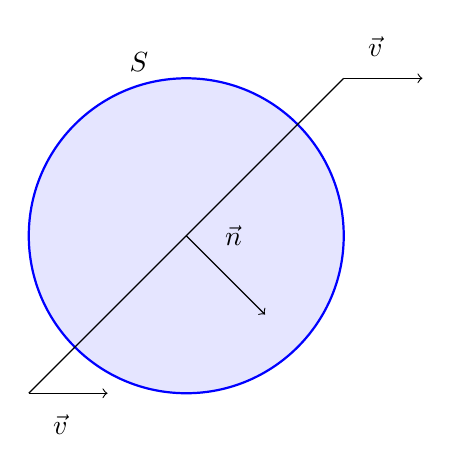
\begin{tikzpicture}[scale=2]
		\draw[thick, blue, fill=blue!10] (0,0) circle(1);
		\draw (-1,-1) -- (1,1);
		\draw[->] (-1,-1) -- (-0.5,-1);
		\draw[->] (1,1) -- (1.5, 1);
		\draw[->] (0,0) -- (0.5,-0.5);
		\node at (1.2,1.2) {$\vec{v}$};
		\node at (-0.8,-1.2) {$\vec{v}$};
		\node at (0.3,-0.0) {$\vec{n}$};
		\node at (-0.3, 1.1) {$\mathfrak{S}$};
	\end{tikzpicture}
	\caption{Aperture problem, figure inspired by \citet{Yazdanbakhsh20111093}. If the line defined by $\vec{n}$ is observed only in the area defined by $\mathfrak{S}$, then any movement along any $\vec{v}$ will be observed as movement along $\vec{n}$.}
	\label{fig:aperture}
\end{figure}

Figure \vref{fig:aperture} tries to illustrate how the aperture problem arises. If the area that are being tracked 
only contains a single edge, then it is impossible to say if there are movement in any direction that is not 
parallel to the normal direction to the edge. This means that tracing a single edge is not favourable, and all 
modern algorithms will try to trace on corners, as a corner by definition is made of at least two non-parallel edges 

\section{Optical flow}
Optical flow is a term that covers the apparent motion of objects, specifically its edges and surfaces 
relative to an observer. The term was first coined for this by James Gibson in the 1940s 
to describe the visual stimulus that animals get from movement\citet{gibson50}.


\subsection{Theory}
The base of optical flow theory is based on the normal flow constraint equation in \eqref{equ:image.constraint}. In equation \eqref{equ:image.constraint}, $I$ is the intensity
at a given point at a given time. It is quite obvious that a normal optical flow problem will be of three dimension as it will include spatial coordinates in addition
to a temporal part. The deltas shown is an indefinite movement in the three dimensions.


\begin{equation}\label{equ:image.constraint}
	I(x,y,t) = I(x + \Delta x, y+ \Delta y, t + \Delta t)
\end{equation}

If the deltas in equation \eqref{equ:image.constraint} is assumed to be small, then the approximation in equation \eqref{equ:image.constraint.taylor} is valid.

\begin{equation}\label{equ:image.constraint.taylor}
	I(x + \Delta x, y+ \Delta y, t + \Delta t) = I(x,y,t) + \frac{\partial I}{\partial x} \Delta x + 
		\frac{\partial I}{\partial y} \Delta y + \frac{\partial I}{\partial t} \Delta t + \mathcal{O}(\partial^2)
\end{equation}

Equation \eqref{equ:image.constraint.taylor} contains a higher order collection term $\mathcal{O}(\partial^2)$. This can be thought of the error in this first order taylor approximation. As
the deltas are assumed small, then the Taylor expansion terms with order higher than one is negligible. 

Substituting equation \eqref{equ:image.constraint} into \eqref{equ:image.constraint.taylor} it is obvious that equation \eqref{equ:taylor.exp} must hold. 
By dividing equation \eqref{equ:taylor.exp} with the change of time we get \eqref{equ:taylor.exp.subs}, where $V_x$ and $V_y$ are the spatial velocities in the 
$x$ and $y$ direction.

\begin{align}
	\frac{\partial I}{\partial x} \Delta x + \frac{\partial I}{\partial y} \Delta y + 
		\frac{\partial I}{\partial t} \Delta t &= 0 \label{equ:taylor.exp} \\
	\frac{\partial I}{\partial x} \frac{\Delta x}{\Delta t} + \frac{\partial I}{\partial y} \frac{\Delta y}{\Delta t} + 
		\frac{\partial I}{\partial t} \frac{\Delta t}{\Delta t} &= \frac{0}{\Delta t} \notag \\
	\frac{\partial I}{\partial x} V_x + \frac{\partial I}{\partial y} V_y + \frac{\partial I}{\partial t}  &= 0 \label{equ:taylor.exp.subs}
\end{align}

By defining the intensity spatial derivatives as $I_x$, $I_y$ and $I_t$, we get equation \eqref{equ:intensity.deriv}. Using the dot product on the derivatives 
leads to equation \eqref{equ:optical.flow}, which is the usual way of writing the optical flow problem.

\begin{align}
	I_x V_x + I_y V_y &= -I_t \label{equ:intensity.deriv} \\
	\nabla I^\top \cdot \vec{V} &= -I_t \label{equ:optical.flow}
\end{align}

Equation \eqref{equ:optical.flow} shows the big problem of optical flow problems. It is a single equation with two unknowns, and is therefore not 
solvable without adding additional constraints to the analysis. The problem is known as the aperture problem, and all of the following algorithms 
introduces some additional condition that infers constraints to the flow problem.

\subsection{Phase correlation}\label{sec:phase.correlation}
As the name of this method implies, this method uses shift and correlation in the phase plane between to frames as a measure of motion. Given that correlation is a global operation,
the method is also image global. The first step is to apply the Fourier transform to both frames, $\textbf{G}_a = \mathcal{F}\{g_a\}$ and $\textbf{G}_b = \mathcal{F}\{g_b\}$. The cross-power spectrum 
can then be calculated with equation \eqref{equ:phase.cross.power}.

\begin{equation}\label{equ:phase.cross.power}
	R = \frac{\textbf{G}_a \circ \textbf{G}_b^\star}{|\textbf{G}_a \textbf{G}_b^\star|}
\end{equation}

By inverse transforming $R$, we get the normalized cross-correlation, $r = \mathcal{F}^{-1}\{R\}$, which can be though of as a 
heat map of the movement between the two frames.

There are however some drawbacks with using the phase correlation method, in addition to the global aspect. The global aspect 
infers smooth and equal movement of all points between the frames. Also, since the Fourier transform is involved. The method has its base 
in the Fourier shift theorem, which implies that the images are assumed to have a circular shift. The case is, however, that the shift 
is more likely to be linear, and this discrepancy gives distortions in the cross-correlation.

\subsection{Lukas-Kanade}\label{sec:lukas-kanade}
The Lucas-Kanade method is a widely used method for providing the needed constraints to solve \eqref{equ:optical.flow}. This method assumes that 
the motion between to frames is small and more or less constant in the neighbourhood of a point, known as the velocity smoothness constraint. 
This means that \eqref{equ:optical.flow} holds for all points within some window
with the point that is being considered. This means that the local velocity vector should satisfy \eqref{equ:lk.local.flow}.

\begin{equation}\label{equ:lk.local.flow}
	\begin{split}
		I_x(q_1)V_x + I_y(q_1)V_y	&= -I_t(q_1) \\
		I_x(q_2)V_x + I_y(q_2)V_y 	&= -I_t(q_2) \\
		&\,\,\, \vdots \\
		I_x(q_N)V_x + I_y(q_N)V_y 	&= -I_t(q_N)
	\end{split}
\end{equation}

Rewriting \eqref{equ:lk.local.flow} on matrix form using the normal $Av = b$ structure, we get the matrices in \eqref{equ:lk.local.flow.mat}.

\begin{equation} \label{equ:lk.local.flow.mat}
A = \begin{bmatrix}
		I_x(q_1) 	& I_y(q_1) \\
		I_x(q_2) 	& I_y(q_2) \\ 
		\vdots 		& \vdots \\
		I_x(q_N)	& I_y(q_N)
	\end{bmatrix} \quad 
v =	\begin{bmatrix}
		V_x \\ V_y
	\end{bmatrix} \quad
b = \begin{bmatrix}
		-I_t(q_1) \\ -I_t(q_2) \\ \vdots \\ -I_t(q_N)
	\end{bmatrix}
\end{equation}

The equation set in \eqref{equ:lk.local.flow.mat} is overdetermined. The Lucas-Kanade method now uses the 
least squares method to find the minimal solution to this set. The system that then must be solved usually takes the 
form of \eqref{equ:lk.local.flow.solv}.

\begin{equation}\label{equ:lk.local.flow.solv}
	v = \left(A^\top A\right)^{-1} A^\top b
\end{equation}

If equation \eqref{equ:lk.local.flow.solv} is expanded back to its original matrices and using sums, we have the system in \eqref{equ:lk.local.flow.solv.full}

\begin{equation}\label{equ:lk.local.flow.solv.full}
	\begin{bmatrix}
		V_x \\ V_y
	\end{bmatrix} = 
	\begin{bmatrix}
		\sum_ i{I_x^2(q_i)} 	 & \sum_i{I_x(q_i)I_y(q_i)} \\
		\sum_i{I_y(q_i)I_x(q_i)} & \sum{I_y^2(q_i)}
	\end{bmatrix}^{-1}
	\begin{bmatrix}
		-\sum_i{I_x(q_i)I_t(q_i)} \\ -\sum_i{I_y(q_i)I_t(q_i)}
	\end{bmatrix}
\end{equation}

\subsection{Horn-Schunck}\label{sec:horn-schunck}
The Horn-Schunck method is another global algorithm\citet{horn80}. It assumes that the flow in a frame is smooth and will minimize any error in this assumption.
It formulates the flow as a energy function on the form \eqref{equ:horn.schunck}, which can be minimized using the corresponding Euler-Lagrange equations in \eqref{equ:horn.schunck.euler} with
$L=\int{E}$.

\begin{equation}\label{equ:horn.schunck}
	E = \int \int \Big ( \big (I_x u + I_y v + I_t\big )^2 + \alpha^2\big (||\nabla u||^2 + ||\nabla v||^2\big ) \Big )\; \mathrm{d}x\,\mathrm{d}y
\end{equation}

\begin{equation}\label{equ:horn.schunck.euler}
	\begin{split}
		\frac{\partial L}{\partial u} - \frac{\partial}{\partial x}\frac{\partial L}{\partial u_x} - \frac{\partial}{\partial y}\frac{\partial L}{\partial u_y} &= 0 \\
		\frac{\partial L}{\partial v} - \frac{\partial}{\partial x}\frac{\partial L}{\partial v_x} - \frac{\partial}{\partial y}\frac{\partial L}{\partial v_y} &= 0
	\end{split}
\end{equation}

The solution to the system in \eqref{equ:horn.schunck} and \eqref{equ:horn.schunck.euler} uses the same arguments as those given in \citet{khalil01} for energy based system analysis.
The full analytical steps and solution can be found in \citet{horn80} which will be omitted here. The result usually takes the form as the iterative equations in \eqref{equ:horn.schunck.solution}.

\begin{equation}\label{equ:horn.schunck.solution}
	\begin{split}
		u^{k + 1} &= \bar{u}^k - \frac{I_x\left(I_x\bar{u}^k + I_y\bar{u}^k + I_t\right)}{\alpha^2 + I_x^2 + I_y^2} \\
		v^{k + 1} &= \bar{v}^k - \frac{I_x\left(I_x\bar{v}^k + I_y\bar{v}^k + I_t\right)}{\alpha^2 + I_x^2 + I_y^2}
	\end{split}
\end{equation}


\cleardoublepage


\chapter{Application of Algorithms}
In this chapter the main algorithms that were covered in chapter \ref{chp:vision} are going to 
be examined in a more practical fashion. The algorithms will 
be prototyped against the navigation scenario in a net.

As mentioned in section \vref{sec:high_def_video_analysis} all implementations done uses the open source \gls{ocv} library. This is done 
through the \gls{python} bindings made available by the project for prototyping, and through the \gls{cpp} API to see how 
the runtime of the algorithms compare. By design, \gls{python} will be slower than the \gls{cpp} versions as \gls{python} is a 
interpreted and \gls{jit} based run time. This means that the \gls{python} runtime needs to perform \gls{marshalling} which 
gives a speed impact.

\section{Optical flow algorithms}

\subsection{Flow fields}
Lucas-Kanade is the main algorithm that tries to identify optical flow by modelling the difference between two frames as a flow field. This algorithm 
is described in section \vref{sec:lukas-kanade}. 

The version of Lucas-Kanade that were implemented is based on the pyramid version of the algorithm. This makes the 
algorithm less computational expensive. The pyramid is built up based on the \verb|cv::goodFeaturesToTrack| function in the OpenCV library. 
This function uses a Canny edge detector to detect features in a frame. This makes use of the fact that edge intersections 
normally does not deform between two frames. Features that are traceable will by that argument be in the 
concave section of two or more intersecting Canny lines.

The initialization of the feature points yields the image in figure \vref{fig:lk_1}. The red circles shows 
where the Canny detector has found strong enough line intersections.

\begin{figure}[htbp]
	\centering
	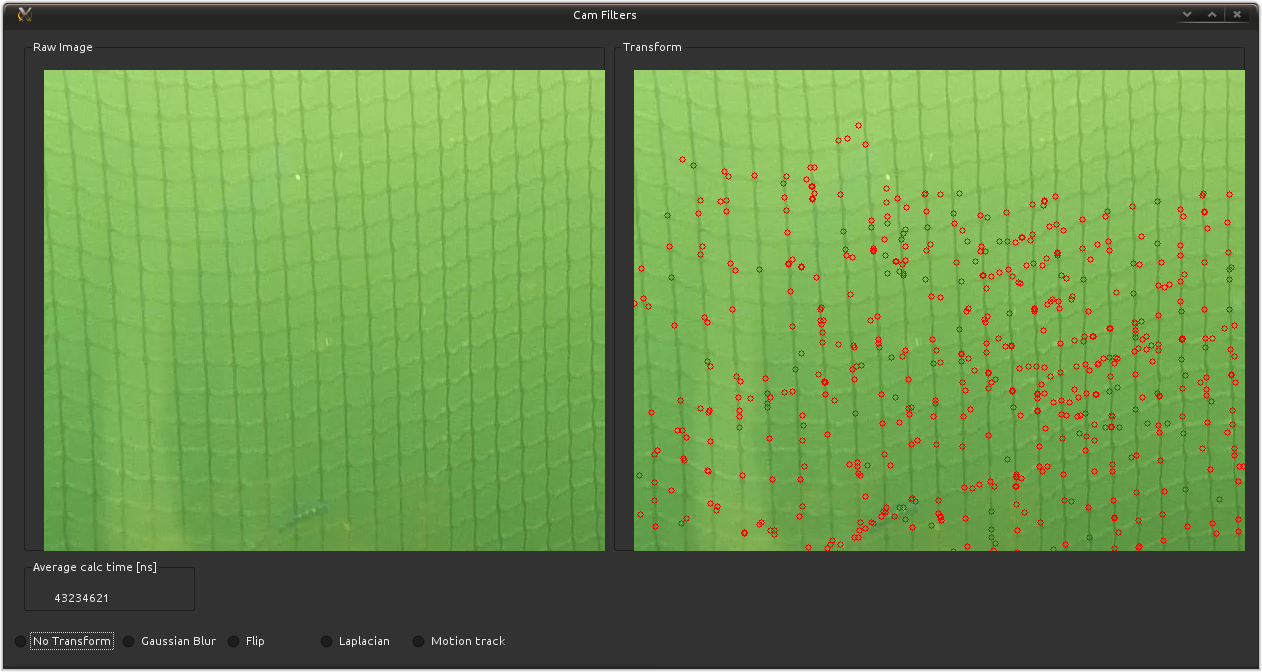
\includegraphics[width=\textwidth]{lk_pyramid_1}
	\caption{Initialization point of Lucas-Kanade. Red dots show the tracking result from the Canny Edge Detector.}
	\label{fig:lk_1}
\end{figure}

The problem with finding good enough features becomes evident after some time. Figure \vref{fig:lk_2} shows the 
tracking result after \SI{1}{\second}. Since the features needs to be constant to be tracked, no new features are found as masks in the net moves 
off the screen. This is mainly rooted in the normal application of algorithms such as this. Normally, the algorithm would be used to track either a single object or 
some discrete number of objects in a stream of frames. 

Applying the Lucas-Kanade algorithm however to the net scenario yields bad results. One reason is that the track points starts to slip on the features 
that were chosen to be tracked. The reason for this is the relative uniformity of the environment, which is not something that the Lucas-Kanade algorithm 
were designed to track. This is rooted in the velocity smoothness constraint mentioned in section \ref{sec:lukas-kanade} 

\begin{figure}
	\centering
	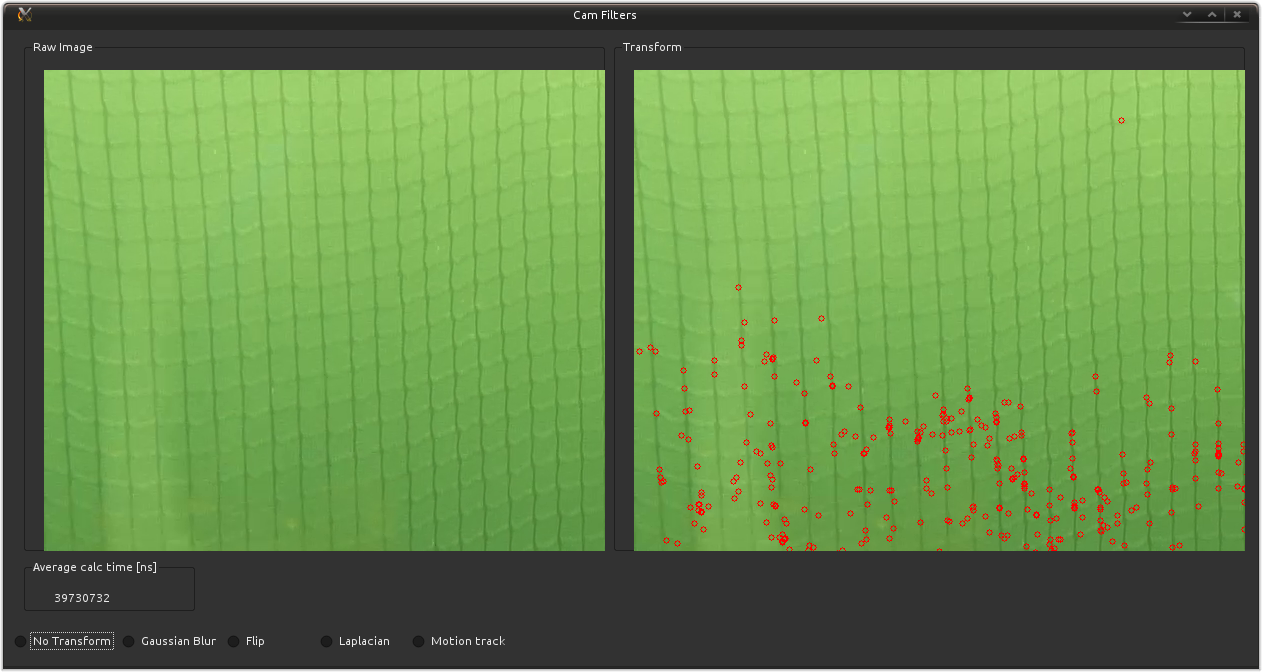
\includegraphics[width=\textwidth]{lk_pyramid_2}
	\caption{1 second of tracking using the Lucas-Kanade algorithm with the initialization from \ref{fig:lk_1}.}
	\label{fig:lk_2}
\end{figure}

\subsection{Energy fields}

\subsubsection{Horn-Schunck}
The main algorithm that uses energy fields to model the flow between two frames is the Horn-Schunck algorithm described in section \vref{sec:horn-schunck}. This 
algorithm has been more or less replaced by the \citet{farnebackSCIA03} algorithm, as described in section \vref{sec:farneback}. 

On this background, the Horn-Schunck 
algorithm were not implemented or tested. 
This is mainly because of the statistical data presented by \citet{farnebackSCIA03} showing that the 
Farnebäck algorithm never gives a worse result than the Horn-Schunck algorithm, while proving to be 
less computational expensive.

\clearpage

\subsubsection{Farnebäck}
Farnebäck became the algorithm with a base in the theory of energy fields that were implemented. This 
is quite a new algorithm in the field of optical flow, but it has proven itself to be 
quite a robust and attractive algorithm. The implementation is based on \citet{farnebackSCIA03} by 
using the \gls{ocv} library.

The image in figure \ref{fig:farneback_1} shows the field calculated 
by the algorithm during linear translation in a realistic scenario. This means 
that even though the majority of movement found goes in the 
downward direction. A close-up view can be seen in figure \ref{fig:farneback_2}.

\begin{figure}[htbp]
	\centering
	
\includegraphics[width=\textwidth]{farneback_1}
	\caption{Using \citet{farnebackSCIA03} to track movement when net is lowered. Each point is the sum of movement in the 
		rectangle which the point is in the centre of that spans to a equidistant grid over the whole image.}
	\label{fig:farneback_1}
\end{figure}

\begin{figure}[htbp]
	\centering
	
\includegraphics[height=\textwidth, angle=90]{farneback_2}
	\caption{Closer look at the output from \citet{farnebackSCIA03} on a subset of masks. Almost uniform flow 
		is detected in the points where the net movement happens. Up direction is to the left in the image.}
	\label{fig:farneback_2}
\end{figure}

Since this algorithm estimates the field in a grid, it can be 
sensitive to weak references and smoothing. A example of real life conditions 
that may lead to a loss of the field in areas with low contrast is shown in 
figure \ref{fig:farneback_3}.

\begin{figure}[htbp]
	\centering
	
\includegraphics[width=\textwidth]{farneback_3}
	\caption{Overview of tracking. Note good tracking in points that contains the vertical parts of the masks and the loss of tracking in 
		the lover left corner.}
	\label{fig:farneback_3}
\end{figure}

Based on how the algorithm calculates the flow, it is also obvious that the Farnebäck algorithm 
is susceptible to other foreground objects that will distort the measurement of the flow for the net. 
This is based in the local grid that this algorithm uses, and it therefore does 
not use some global measurement to detect the mean flow. These features can be seen in figure \ref{fig:farneback_dist_1} and 
\ref{fig:farneback_dist_2}.

\begin{figure}[htbp]
	\centering
	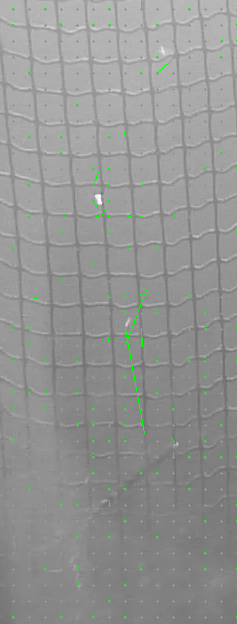
\includegraphics[height=\textwidth, angle=90]{farneback_distortion_1}
	\caption{Showing \citet{farnebackSCIA03} tracking other unwanted objects in the stream. Here some small air bubble are being tracked. 
		Upwards direction is to the left in the image.}
	\label{fig:farneback_dist_1}
\end{figure}

\begin{figure}[htbp]
	\centering
	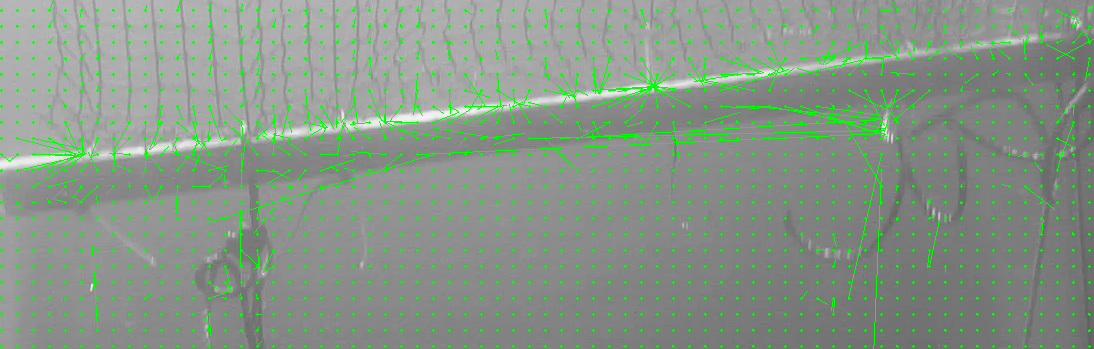
\includegraphics[width=\textwidth]{farneback_distortion_2}
	\caption{Showing \citet{farnebackSCIA03} tracking the bottom line of the rig. Multiple big distortions.}
	\label{fig:farneback_dist_2}
\end{figure}

The hard distortions seen if figure \ref{fig:farneback_dist_1} and 
\ref{fig:farneback_dist_2} stems from the intended use 
of the algorithm. It is optimized to find either global flow when 
the image only contains background, or to track objects in the foreground. 

The Farnebäck algorithm were tested on a sample video. The movement detected by
the algorithm has been plotted in figure \vref{fig:farneback_move}. Note that 
the dimensions for the movement are related by 
some scaling factor to the real movement in the image stream.

\begin{figure}[htbp]
    \centering
    \subfloat[Result of the Farnebäck algorithm detected movement on a sample video.]
    	{\label{fig:farneback_move_1}{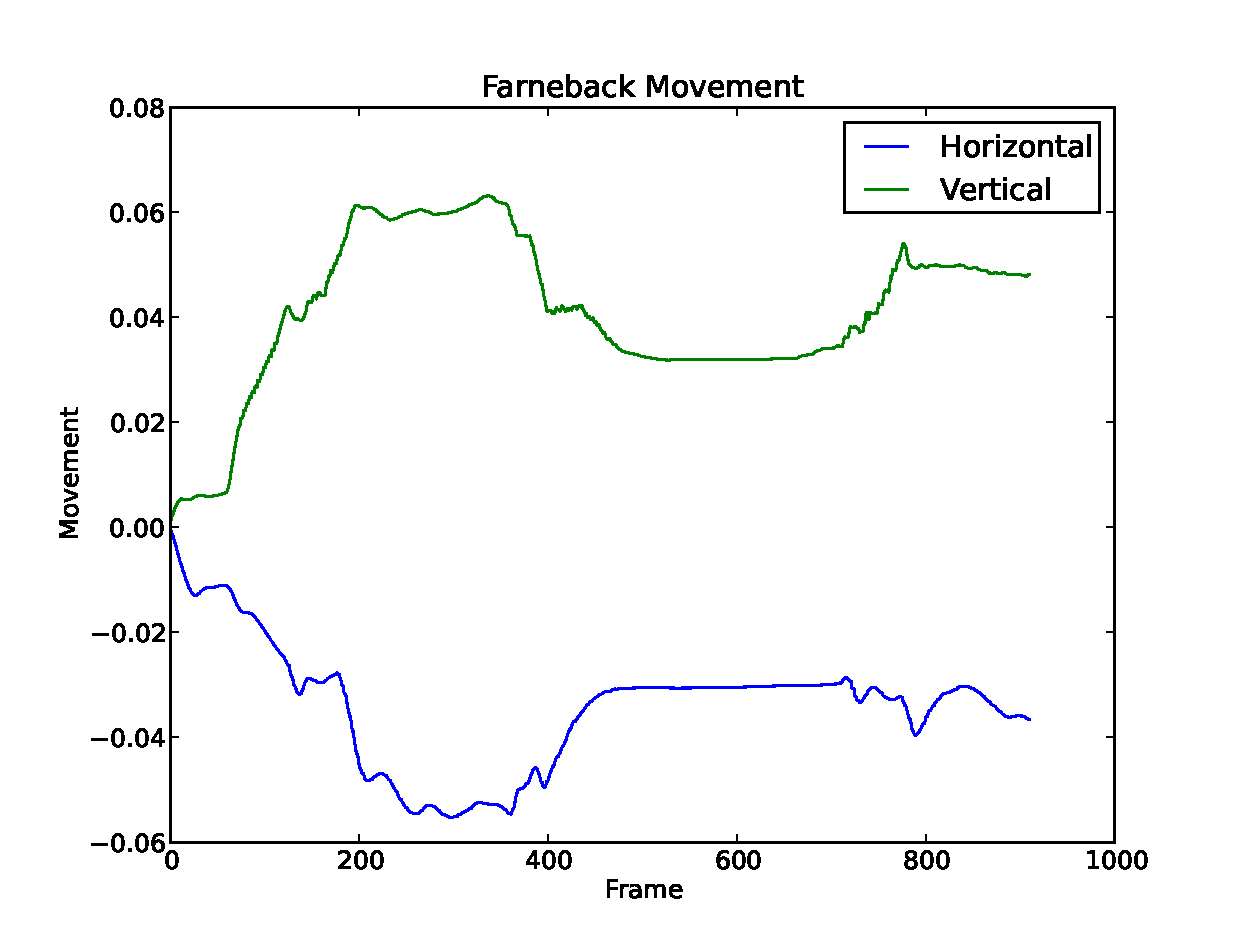
\includegraphics[width=0.8\textwidth]{farneback_move_1}}}
    \\
	\subfloat[Result of the Farnebäck algorithm detected movement on a sample video, horizontal position plotted against vertical position.]
		{\label{fig:farneback_move_2}{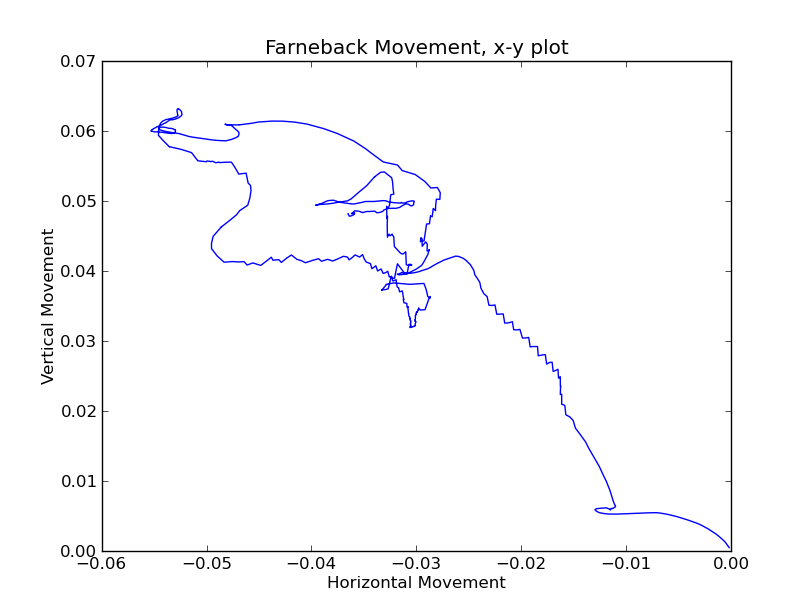
\includegraphics[width=0.8\textwidth]{farneback_move_2}}}
	\caption{Using the Farnebäck algorithm on a sample video. 
		Shown as position vs frame (\ref{fig:phase_run_1}) and x-position vs y-position (\ref{fig:phase_run_2}).}
	\label{fig:farneback_move}
\end{figure}

\clearpage

\subsection{Line tracing}
The use of Hough Transforms was tested by \citet{carlsen10} to detect the net and masks in the net. His trials were initially done in a 
static scenario with the net held in place by a metal frame. He showed that it was possible to find the lines describing the mask 
structure using the normal Hough Transform by setting strict parameters on the minimum distance between detected lines under those conditions.
It proved however to be much worse to get stable readings during his field test, and 

The image in figure \vref{fig:hl_1} shows the results of the normal Hough Transform on the net suspended in free water. Due to the 
movement of the net, and the folding seen in figure \ref{fig:hl_1} the transform fails to find a consistent number of lines. When  
the net starts moving up as shown in figure \ref{fig:hl_2} it seems as most of the lines that were found in figure \ref{fig:hl_1} 
is being tracked correctly. However, as the Hough Transform generates a new set of lines for each image this is not an assumption 
that generally holds. 

\begin{figure}[htbp]
	\centering
	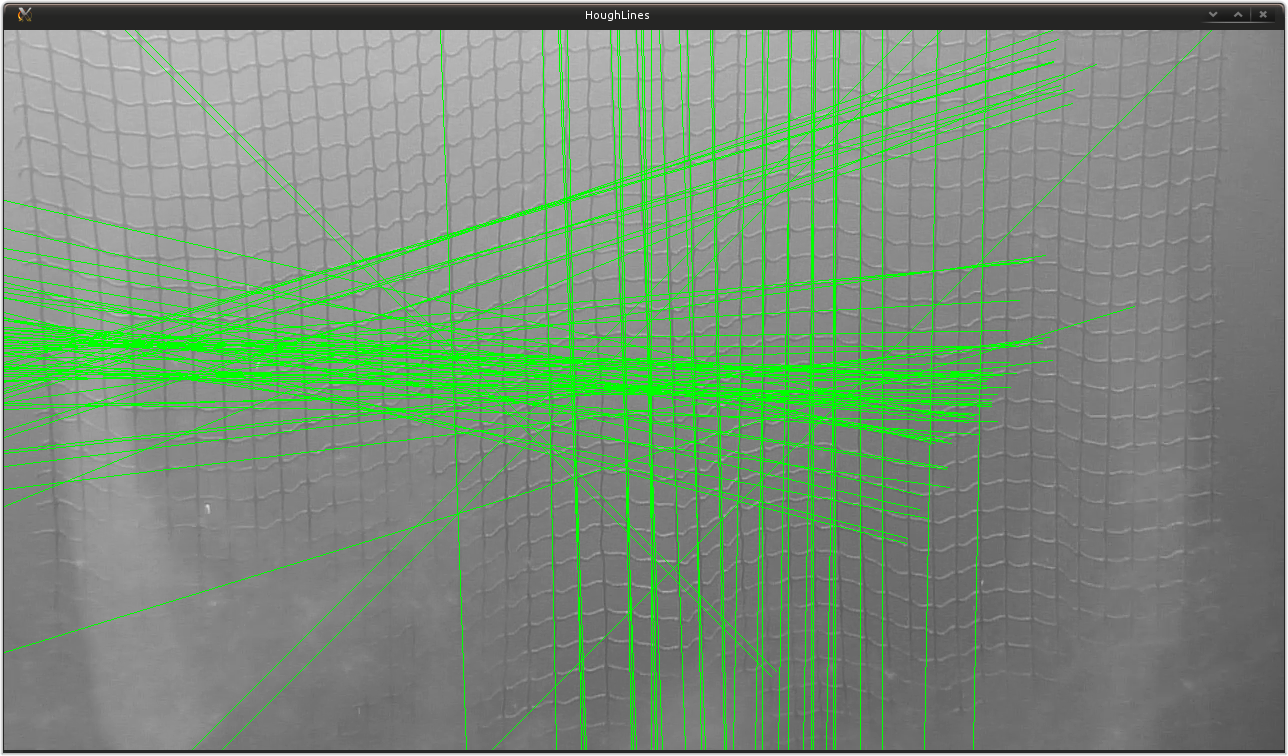
\includegraphics[width=\textwidth]{houghlines_1}
	\caption{Initial result of the Hough Line Transform on a net at rest}
	\label{fig:hl_1}
\end{figure}

\begin{figure}[htbp]
	\centering
	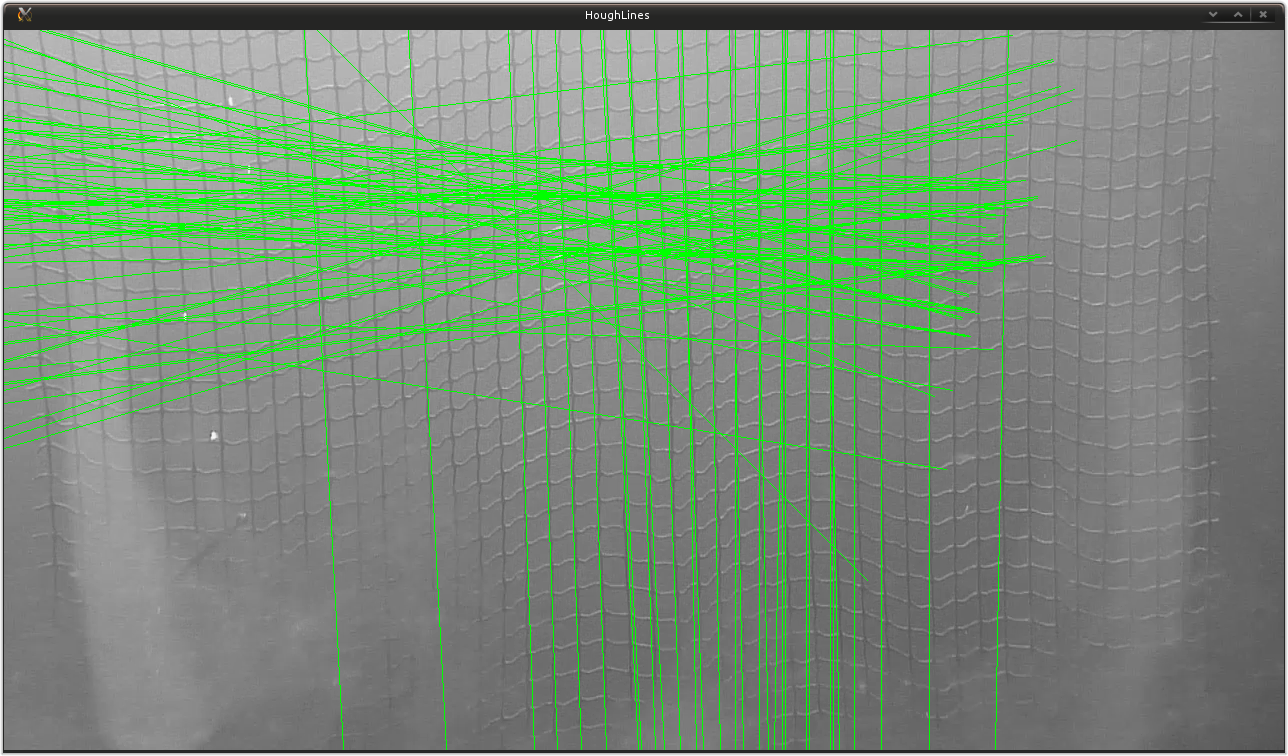
\includegraphics[width=\textwidth]{houghlines_2}
	\caption{Result of the Hough Line Transform when the net is moving}
	\label{fig:hl_2}
\end{figure}

According to section \vref{sec:hough.transform.prob} the Probabilistic Hough transform would be a better choice in the
environment shown in figure \ref{fig:hl_1}. This comes from the design of the algorithm to not 
assume that lines are straight for the duration of the lines. Using the probabilistic properties from section \ref{sec:hough.transform.prob} 
the image in figure \vref{fig:hl_p_1} were obtained. This is from the same sequence as figure \ref{fig:hl_1}. The image in figure \ref{fig:hl_p_2}
is from the same sequence as figure \ref{fig:hl_2}, and shows how the probabilistic transform detects lines during movement.

\begin{figure}[htbp]
	\centering
	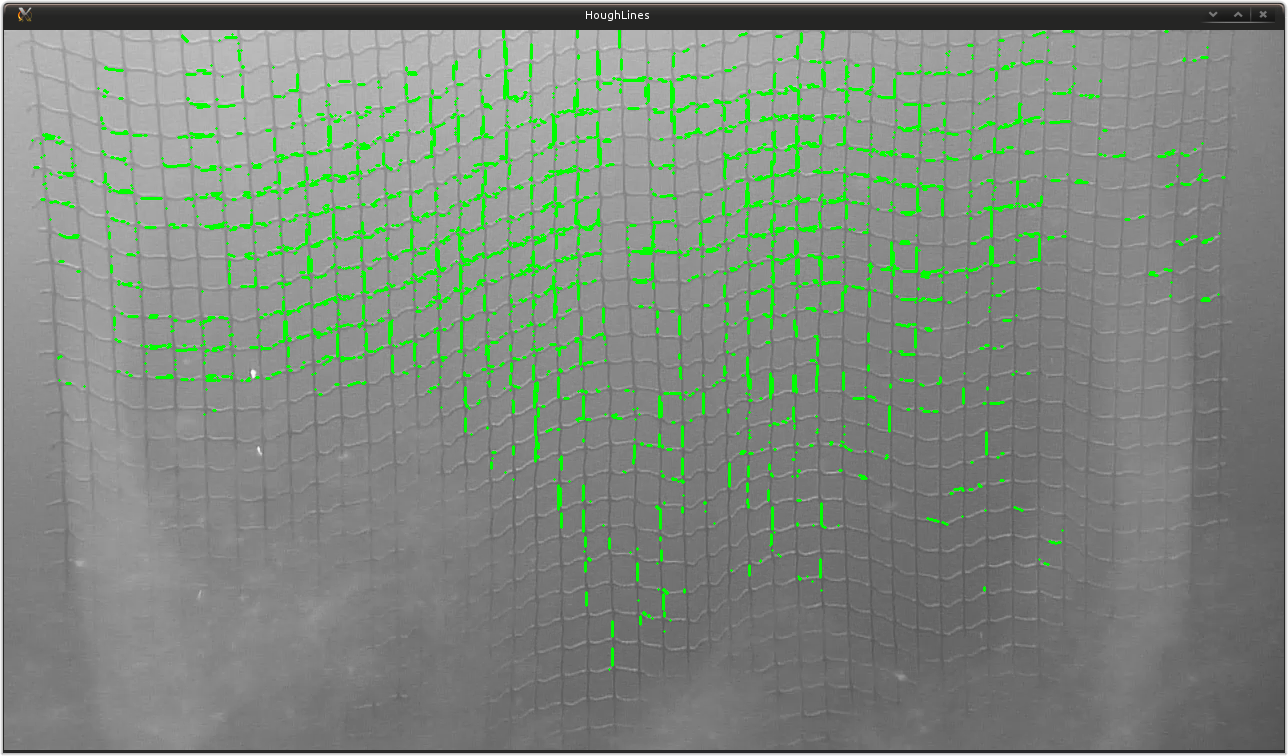
\includegraphics[width=\textwidth]{houghlines_probabilistic_1}
	\caption{Initial result of the Probabilistic Hough Line Transform on a net at rest}
	\label{fig:hl_p_1}
\end{figure}

\begin{figure}[htbp]
	\centering
	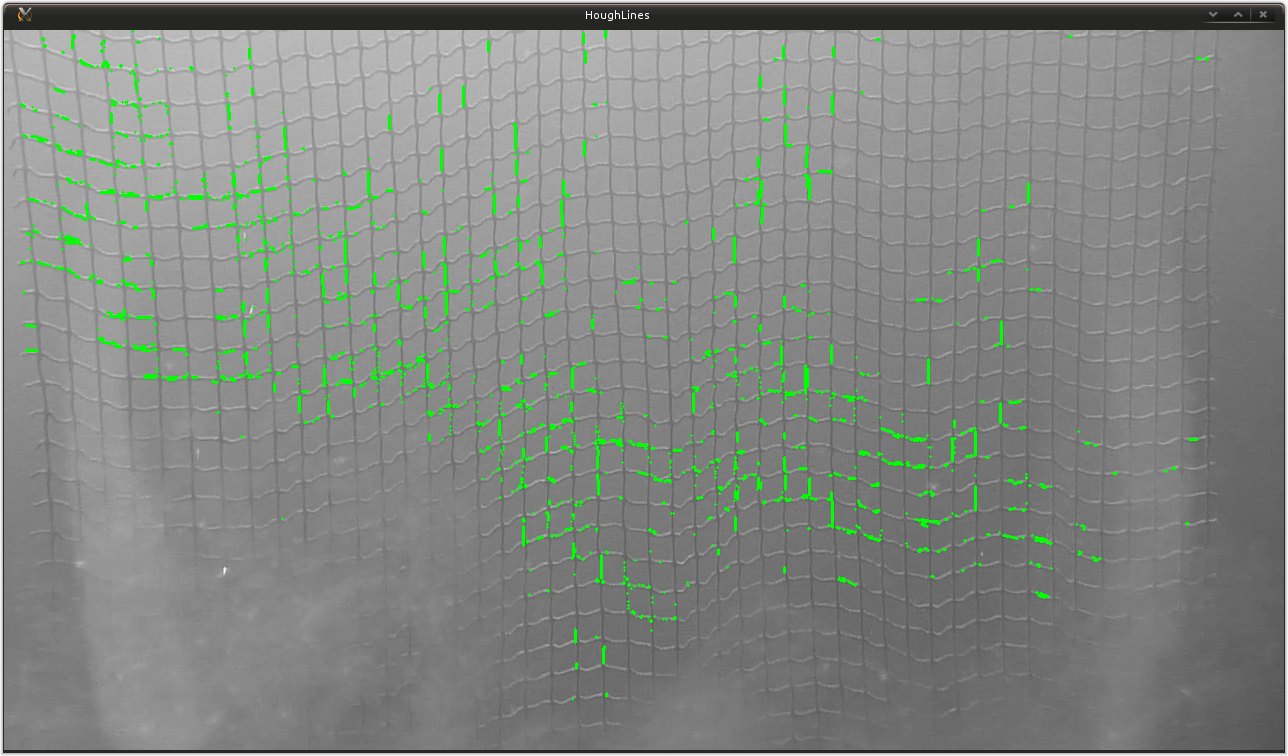
\includegraphics[width=\textwidth]{houghlines_probabilistic_2}
	\caption{Result of the Probabilistic Hough Line Transform when the net is moving}
	\label{fig:hl_p_2}
\end{figure}

\clearpage

\subsection{Phase correlation}
The Phase Correlation algorithm that were described in section \vref{sec:phase.correlation} were also tested. This 
is one of the older methods of finding flow, and it is mainly designed to find the linear translation between two frames.
The use of a phase plane makes the algorithm extremely resilient to noise in the image. This is in sharp contradiction 
to other algorithms that work in the spatial domain.

\begin{figure}[htbp]
    \centering
    \subfloat[Result of Phase Correlation detected movement on a sample video.]
    	{\label{fig:phase_run_1}{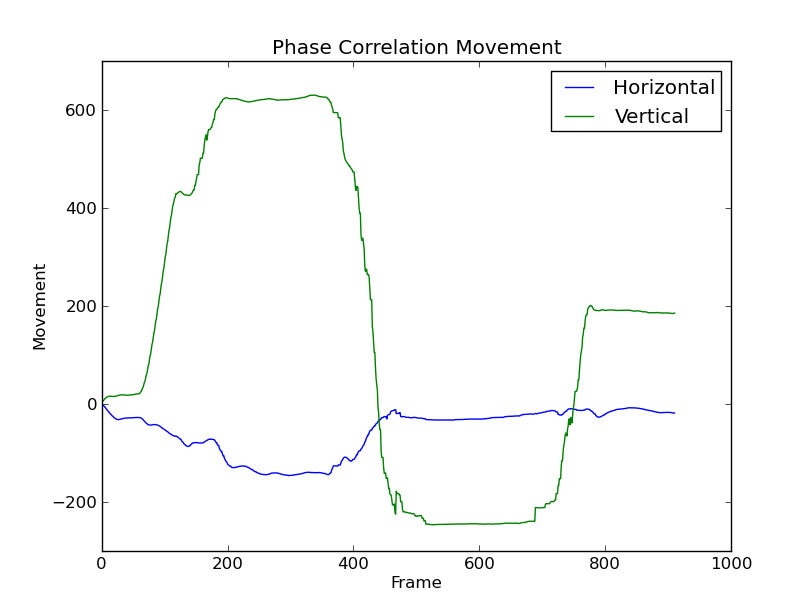
\includegraphics[width=0.8\textwidth]{phase_run_1}}}
    \\
	\subfloat[Result of Phase Correlation detected movement on a sample video, horizontal position plotted against vertical position.]
		{\label{fig:phase_run_2}{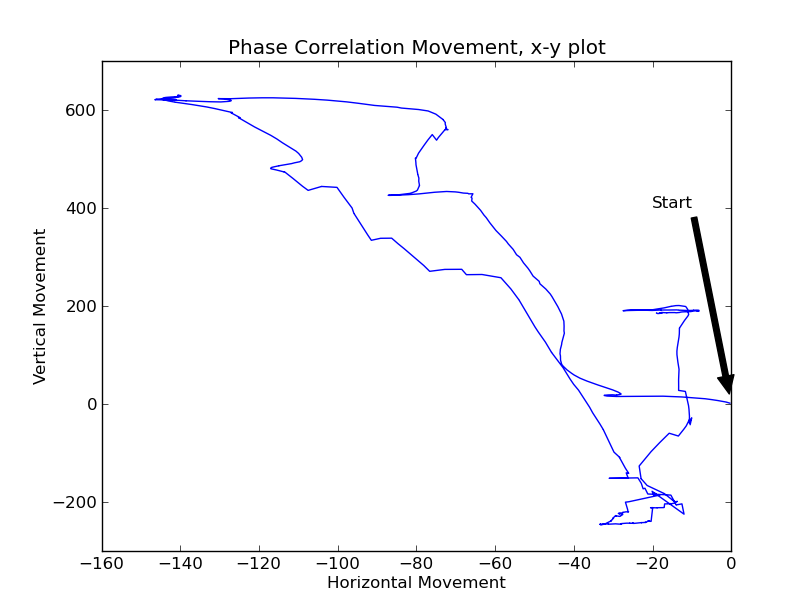
\includegraphics[width=0.8\textwidth]{phase_run_2}}}
	\caption{Using Phase Correlation on a sample video. 
		Shown as position vs frame (\ref{fig:phase_run_1}) and x-position vs y-position (\ref{fig:phase_run_2}).}
	\label{fig:phase_run}
\end{figure}

The output from the phase correlation algorithm is the primary detected movement between two frames, and some 
statistical data about the detected movement. This means that it is easily 
plotted as shown in figure \ref{fig:phase_run}. 

The figures in figure \ref{fig:phase_run} shows the 
same video sequence plotted in two different ways. Figure \ref{fig:phase_run_1} shows the two 
different dimensions of the video and how it is detected to move during the full duration of the stream. This gives a temporal 
view of how the movement progresses. Figure \ref{fig:phase_run_2} shows a polar plot of the same, where the horizontal and vertical 
components  This plot loses the temporal component, but it shows a trace of the 
movement of the net. 

\cleardoublepage


\chapter{Field Tests}\label{ch:field_test}

Computer Vision algorithms can only give as good result as the source videostream that it is 
being fed. After talking a bit to SINTEF, some test videos were provided by them. However, as seen in figure 
\vref{fig:sintef_not_1}, the quality leaves much to be desired. The video provided had a resolution 
of $854 \times 480$ pixels with big black box padding around it. This does not only make 
the video unsuitable for us in a computer vision algorithm, but it also means that the video 
probably is upscaled quite a bit.

Due to the poor nature of the quality of the video it was decided early on that 
a field test was needed, since we were going to use equivalent hardware as to what is available on the ROV. 

\begin{figure}[htbp]
	\centering
	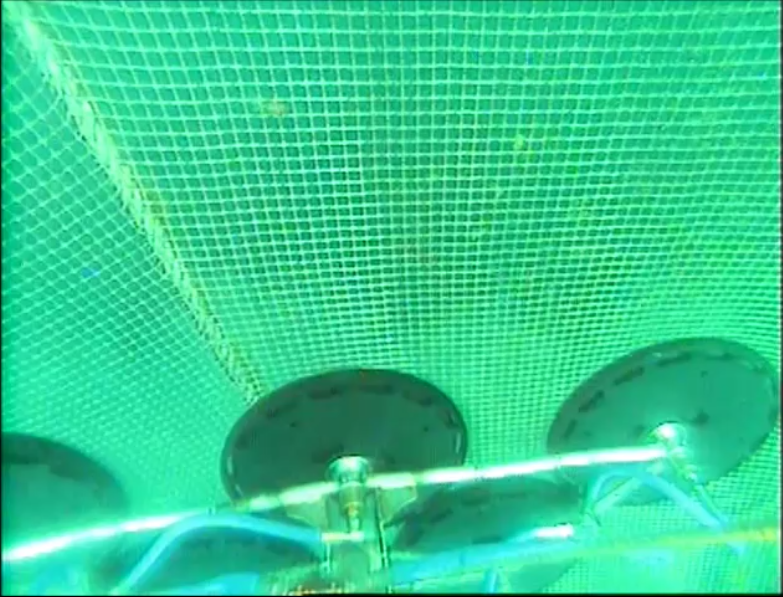
\includegraphics[width=0.9\textwidth]{sintef_not_video_1}
	\caption{Original video provided by SINTEF}
	\label{fig:sintef_not_1}
\end{figure}

\section{SINTEF DVL Test}
This lead to us helping SINTEF out with a doppler velocity log test using a rig for controlling 
the movement of the \todo{not som i garn?}. As a favour for us helping out, we 
got to lend the rig at a later time when our hardware were ready to do a field test. 

During this test, we learned enough ab the rig and operation of it that we should be able to operate 
it ourselves.

\begin{figure}[htbp]
	\centering
	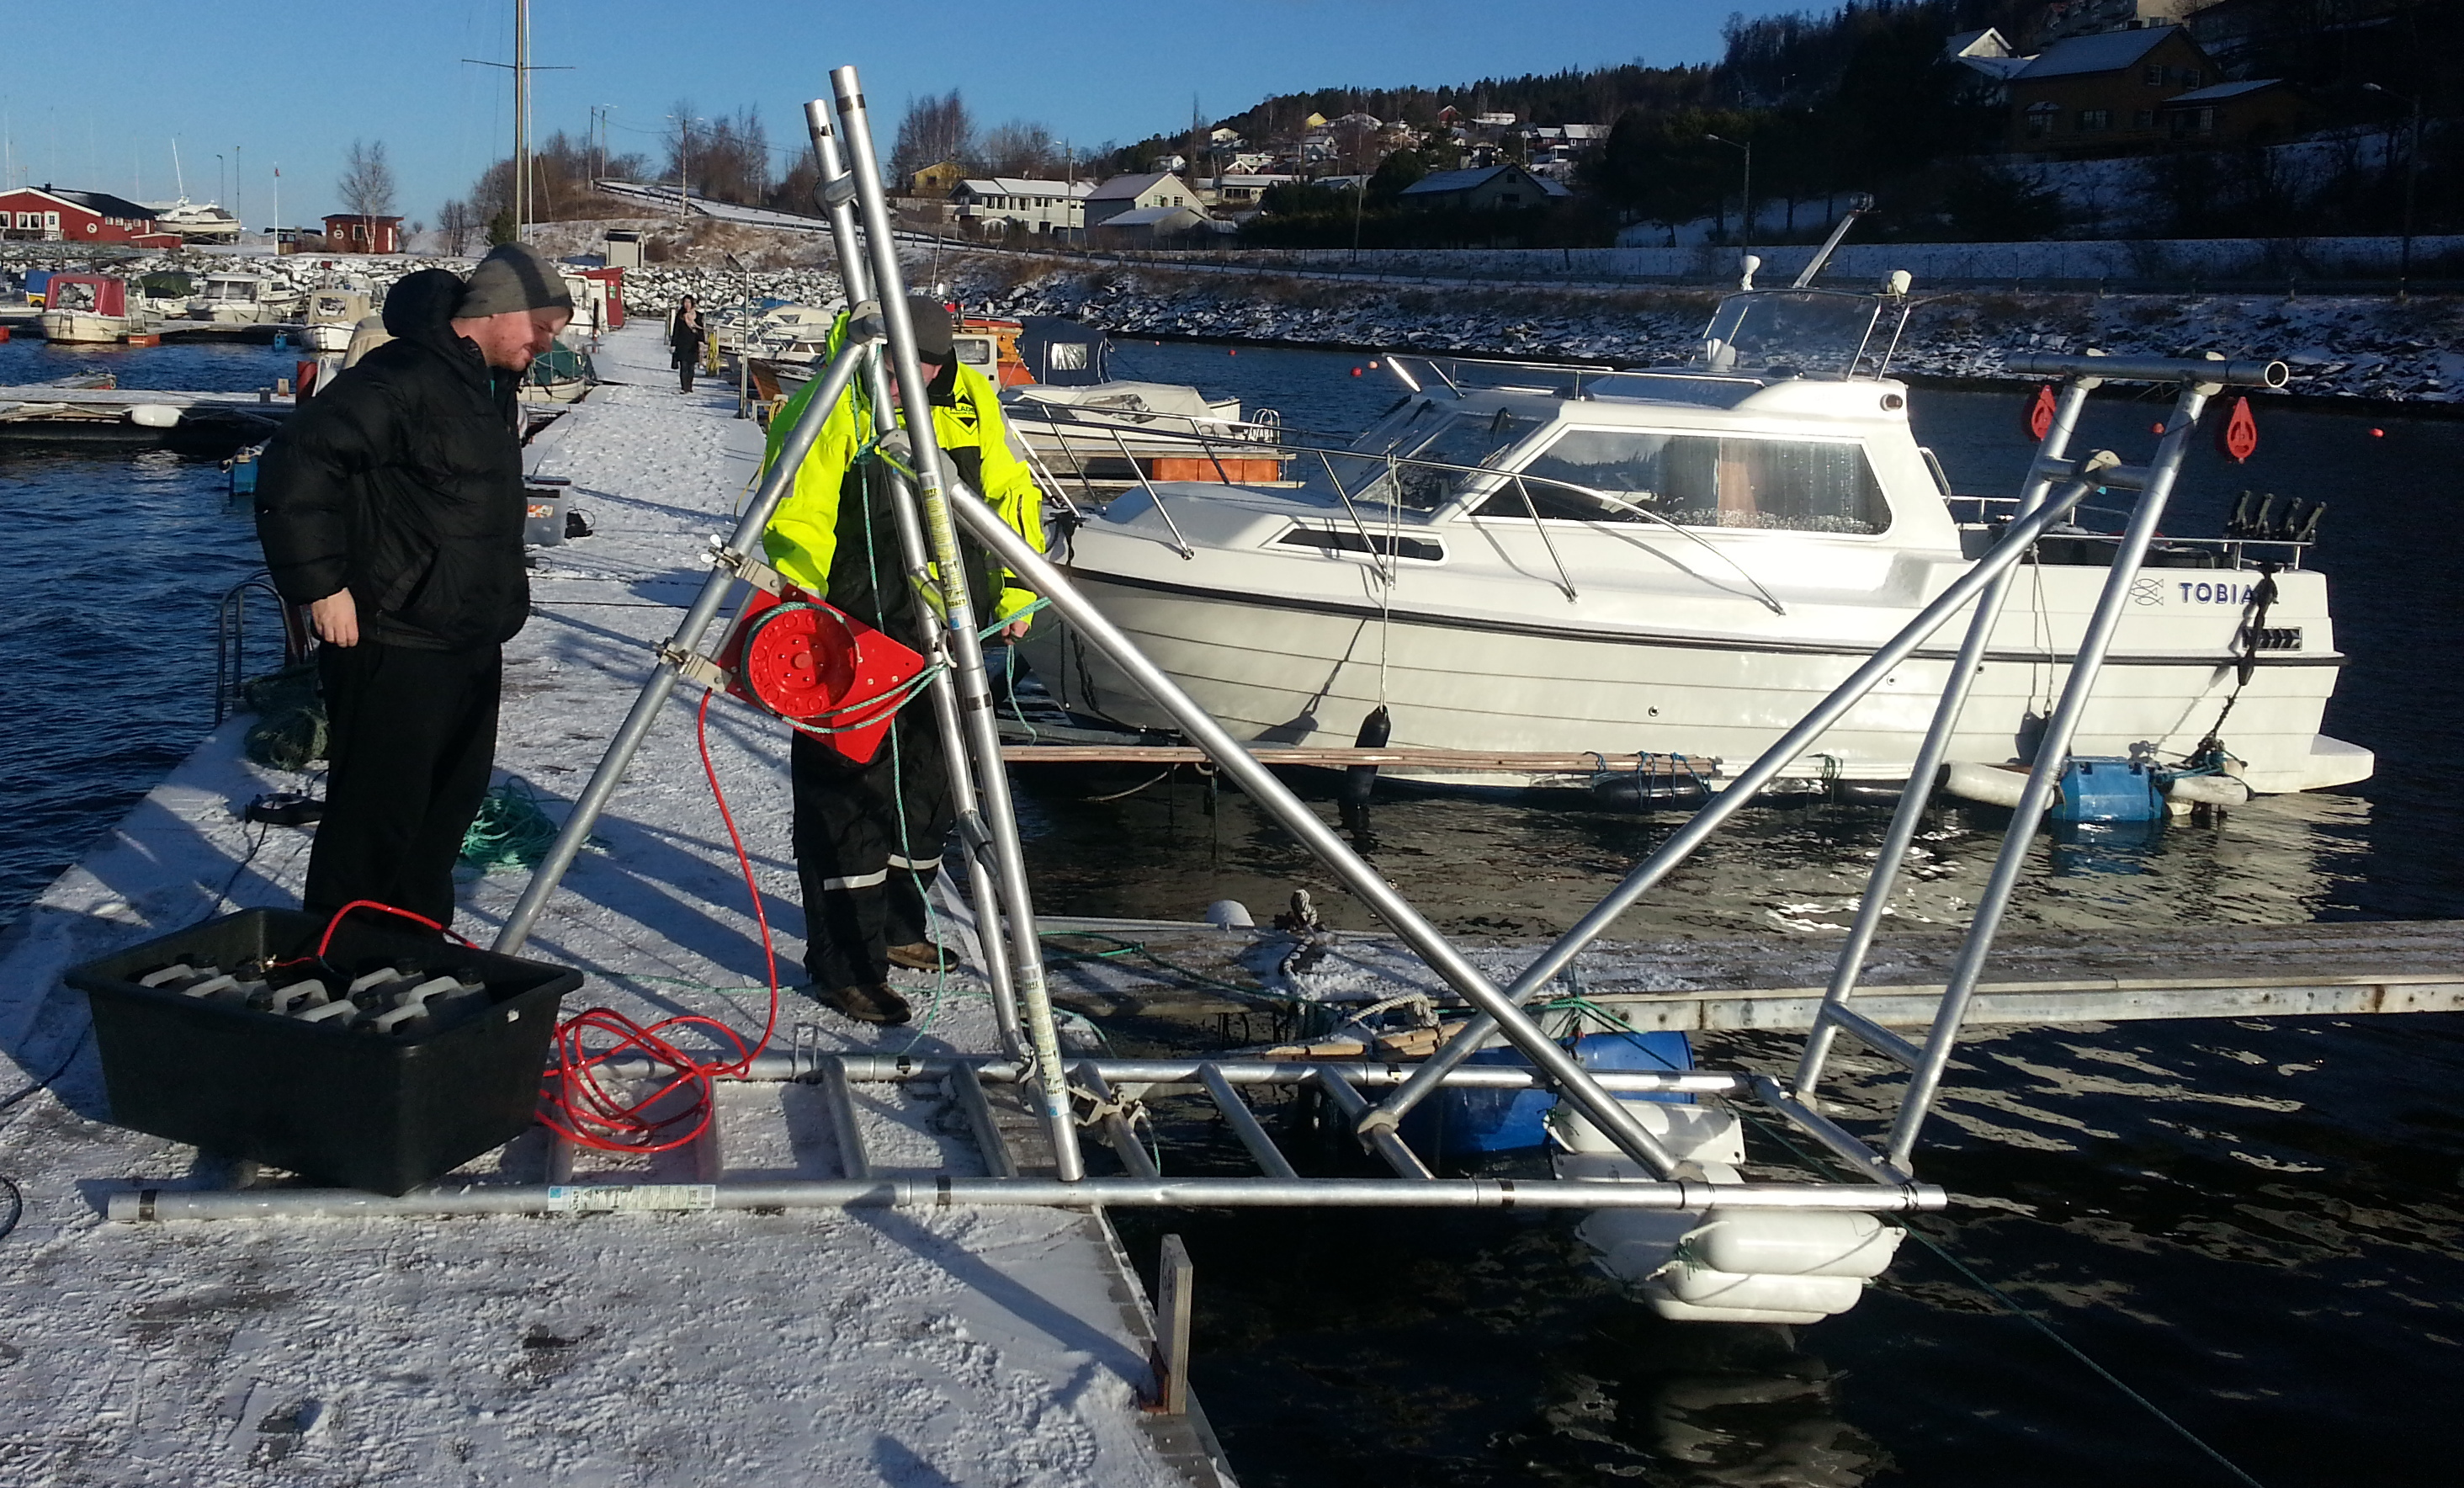
\includegraphics[width=0.9\textwidth]{rig1}
	\caption{Field test for SINTEF using DVL}
	\label{fig:test_dvl}
\end{figure}

\section{HD Video Test}

\begin{figure}[htbp]
	\centering
	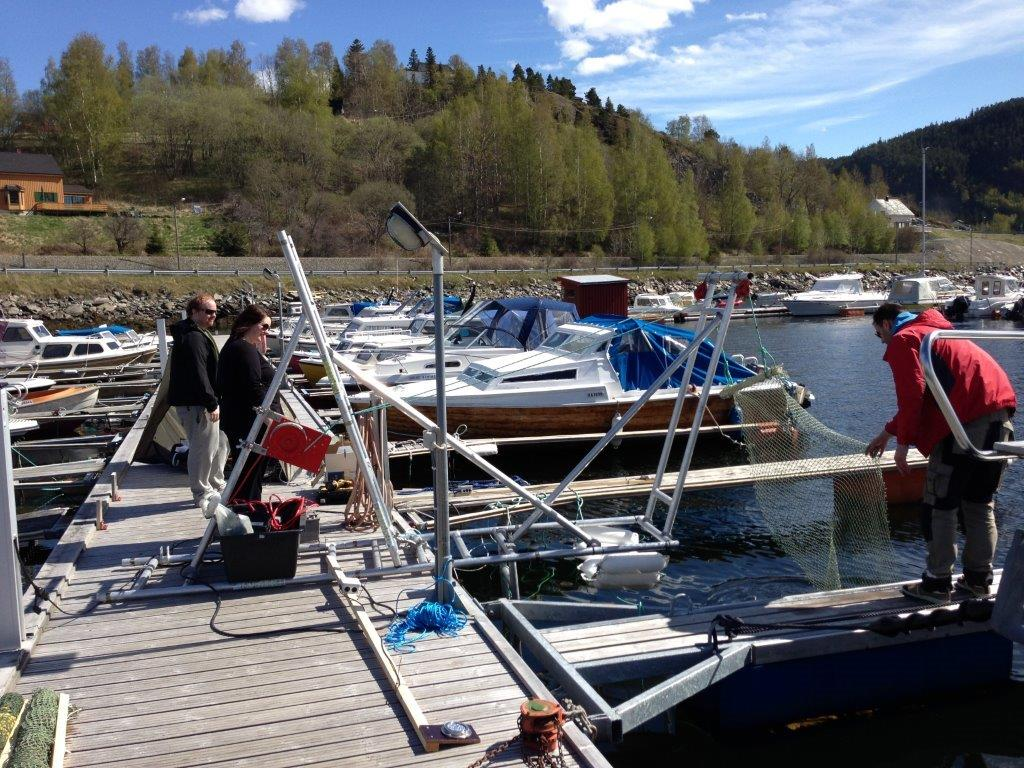
\includegraphics[width=0.9\textwidth]{rig2}
	\caption{Field test}
	\label{fig:test_hd}
\end{figure}

The rig was configured to mimic the approximate distance to the net 
in figure \vref{fig:sintef_not_1}. We were however not able to tilt the camera to 
an angle due to environmental constraint in a anchor chain situated below the camera.
We approximated the distance between the ROV and the net in figure \vref{fig:sintef_not_1} to be 
\SI{1.5}{\metre}. This lead to a the image in \vref{fig:test_hd_referanse}

\begin{figure}[htbp]
	\centering
	
\includegraphics[width=0.9\textwidth]{hd_not_all}
	\caption{View from \SI{1.5}{\metre}}
	\label{fig:test_hd_referanse}
\end{figure}

Comparing image \vref{fig:test_hd_referanse} and \vref{fig:sintef_not_1}, it seems that the 
top row of masks is approximately the same in both images. Due to the tilt of the 
camera in image \ref{fig:sintef_not_1} we get a prominent vanishing point in that image. There 
are also some growing on the net in \ref{fig:sintef_not_1}, which of obvious reasons does not appear 
in \ref{fig:test_hd_referanse}.

\begin{figure}[htbp]
	\centering
	
\includegraphics[width=0.9\textwidth]{hd_not}
	\caption{Field test}
	\label{fig:test_hd_clip}
\end{figure}

\cleardoublepage{}


\chapter{System Implementation}


\section{Hardware Setup}

\subsection{Camera}

\subsection{HD-SDI Interface Card}
The HD-SDI card can be mounted onto a small bracket on the back of the camera. This gives a small 
footprint for the unit. The card is mounted as shown in figure \ref{fig:hd-sdi.card}, where all the connectors are described in 
the figure caption.

The interface has a couple of different functions in the setup. Mainly it does the conversion and 
packing of the LVDS signal from the camera into HD-SDI according to both the HD-SDI protocol and the electrical specification. 
The video data is then available on a MCX7 connector which can be connected to normal BNC using a provided adapter.

There are also a big flat flex cable between the camera and the interface card. This cable is mainly used for sending and receiving the VISCA commands 
to and from the camera. In this situation the interface card provides a level translator so that the signal can be connected directly to a serial 
port on a computer. This serial signal is available on a breakout cable, together with ground references and the analog video outputs from the camera. 

The card also has a single status led to indicate what operating mode the HD-SDI bus is in. On startup the led will be red. This means that 
the video input can not be streamed out to the HD-SDI interface. This usually resolves itself during the setup of the HD-SDI interface between the 
card and the recipient on the other side of the cable. When the setup process is completed, the led will change to green indicating that 
the card is now streaming data. 

During power up, the camera will close and open the iris. This indicates that at least power is getting through. During HD-SDI setup, the camera 
will continue to do this, and it will make clicking sounds. This is a good way of getting feedback without having to constantly 
looking at the interface card.

\begin{figure}
 	\centering
 	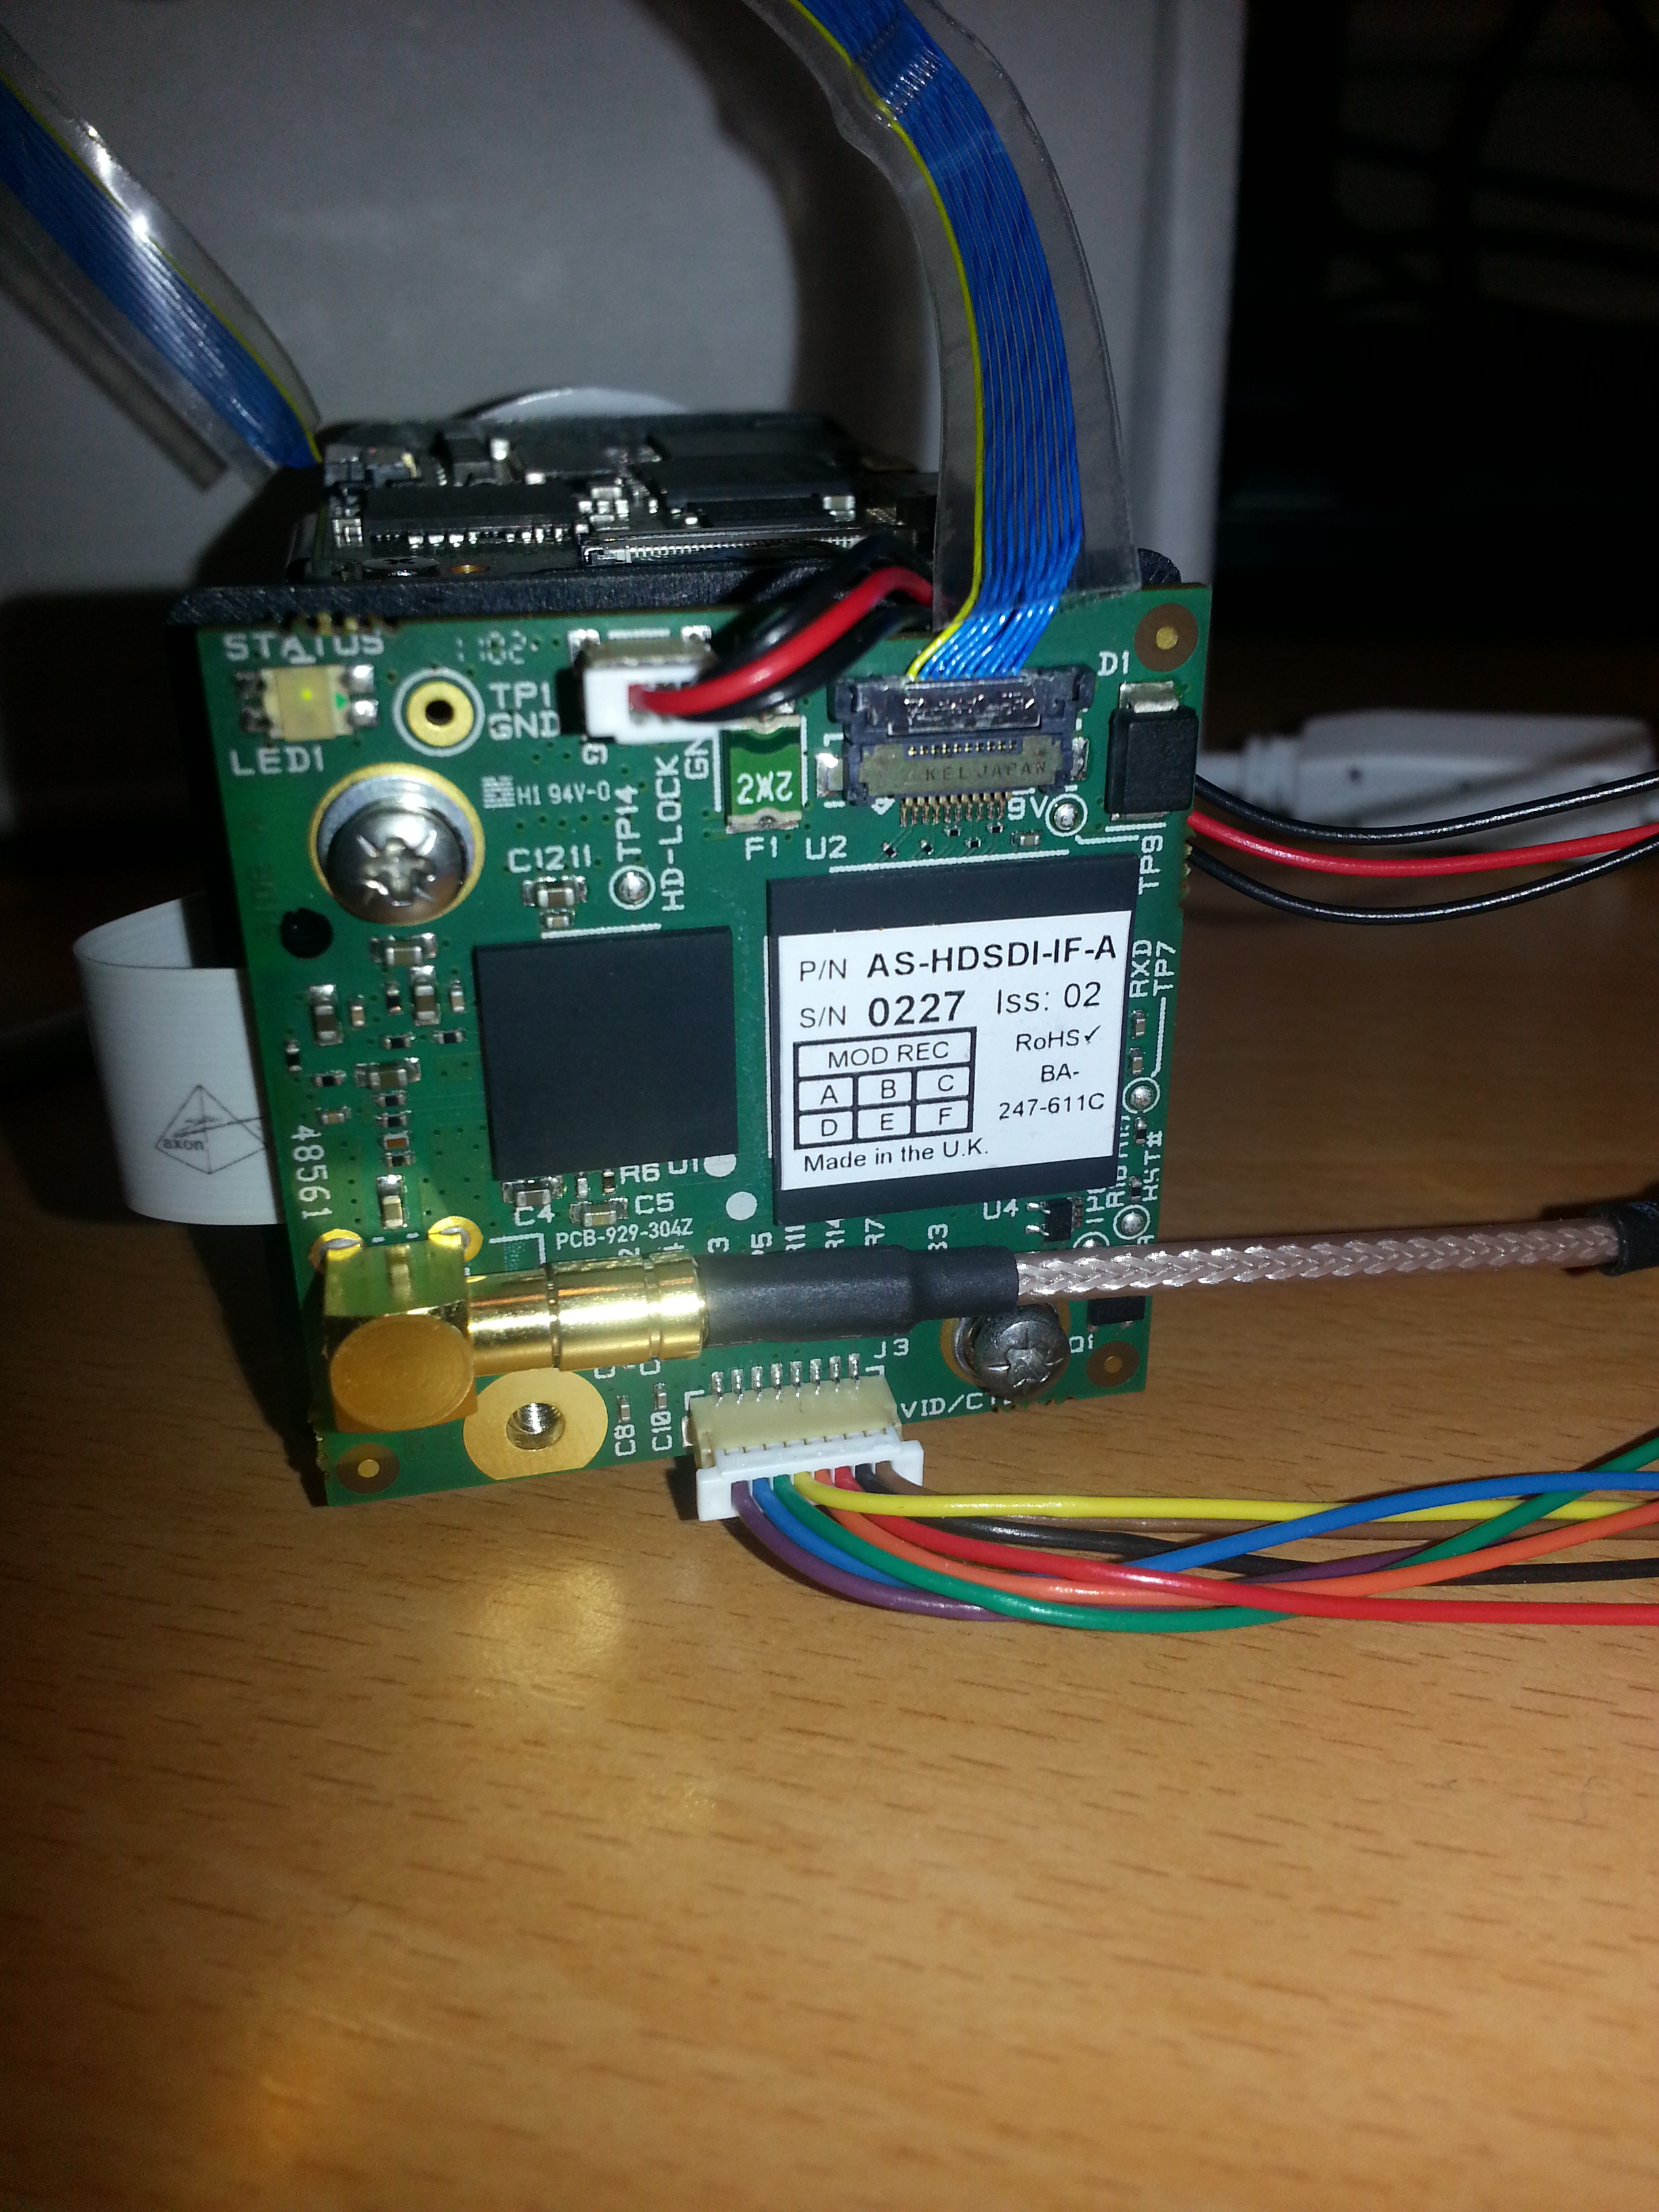
\includegraphics[width=0.94\textwidth]{em1571_real}
 	\caption{EM15710 connected to the camera. Blue flat cable on the top is LVDS from camera. Gray flat flex to the left contains 
 		analog HD, communication and power to the camera. Multicolor molex in the bottom middle contains the analog video signals and level translated communication signals. Molex on the top is power. Gold MCX/BNC is HD-SDI out. Status led on the top left corner is red during signal locking and green during normal operation.}
 	\label{fig:hd-sdi.card}
\end{figure}

\subsection{Underwater Housing}\todo{Add better spec}
As the camera needs to be submerged in water, a waterproof housing for the camera was made by the mechanical workshop at the institute. The housing can 
be seen in figure \vref{fig:housing}. The housing is made up of a tube of clear acrylic plastic with two end pieces. The back piece also
has a sliding bracket that the camera can be mounted to. It also has two nipples for the two cables that is going to carry the video signal and 
the power and control signals. 

\begin{figure}
 	\centering
 	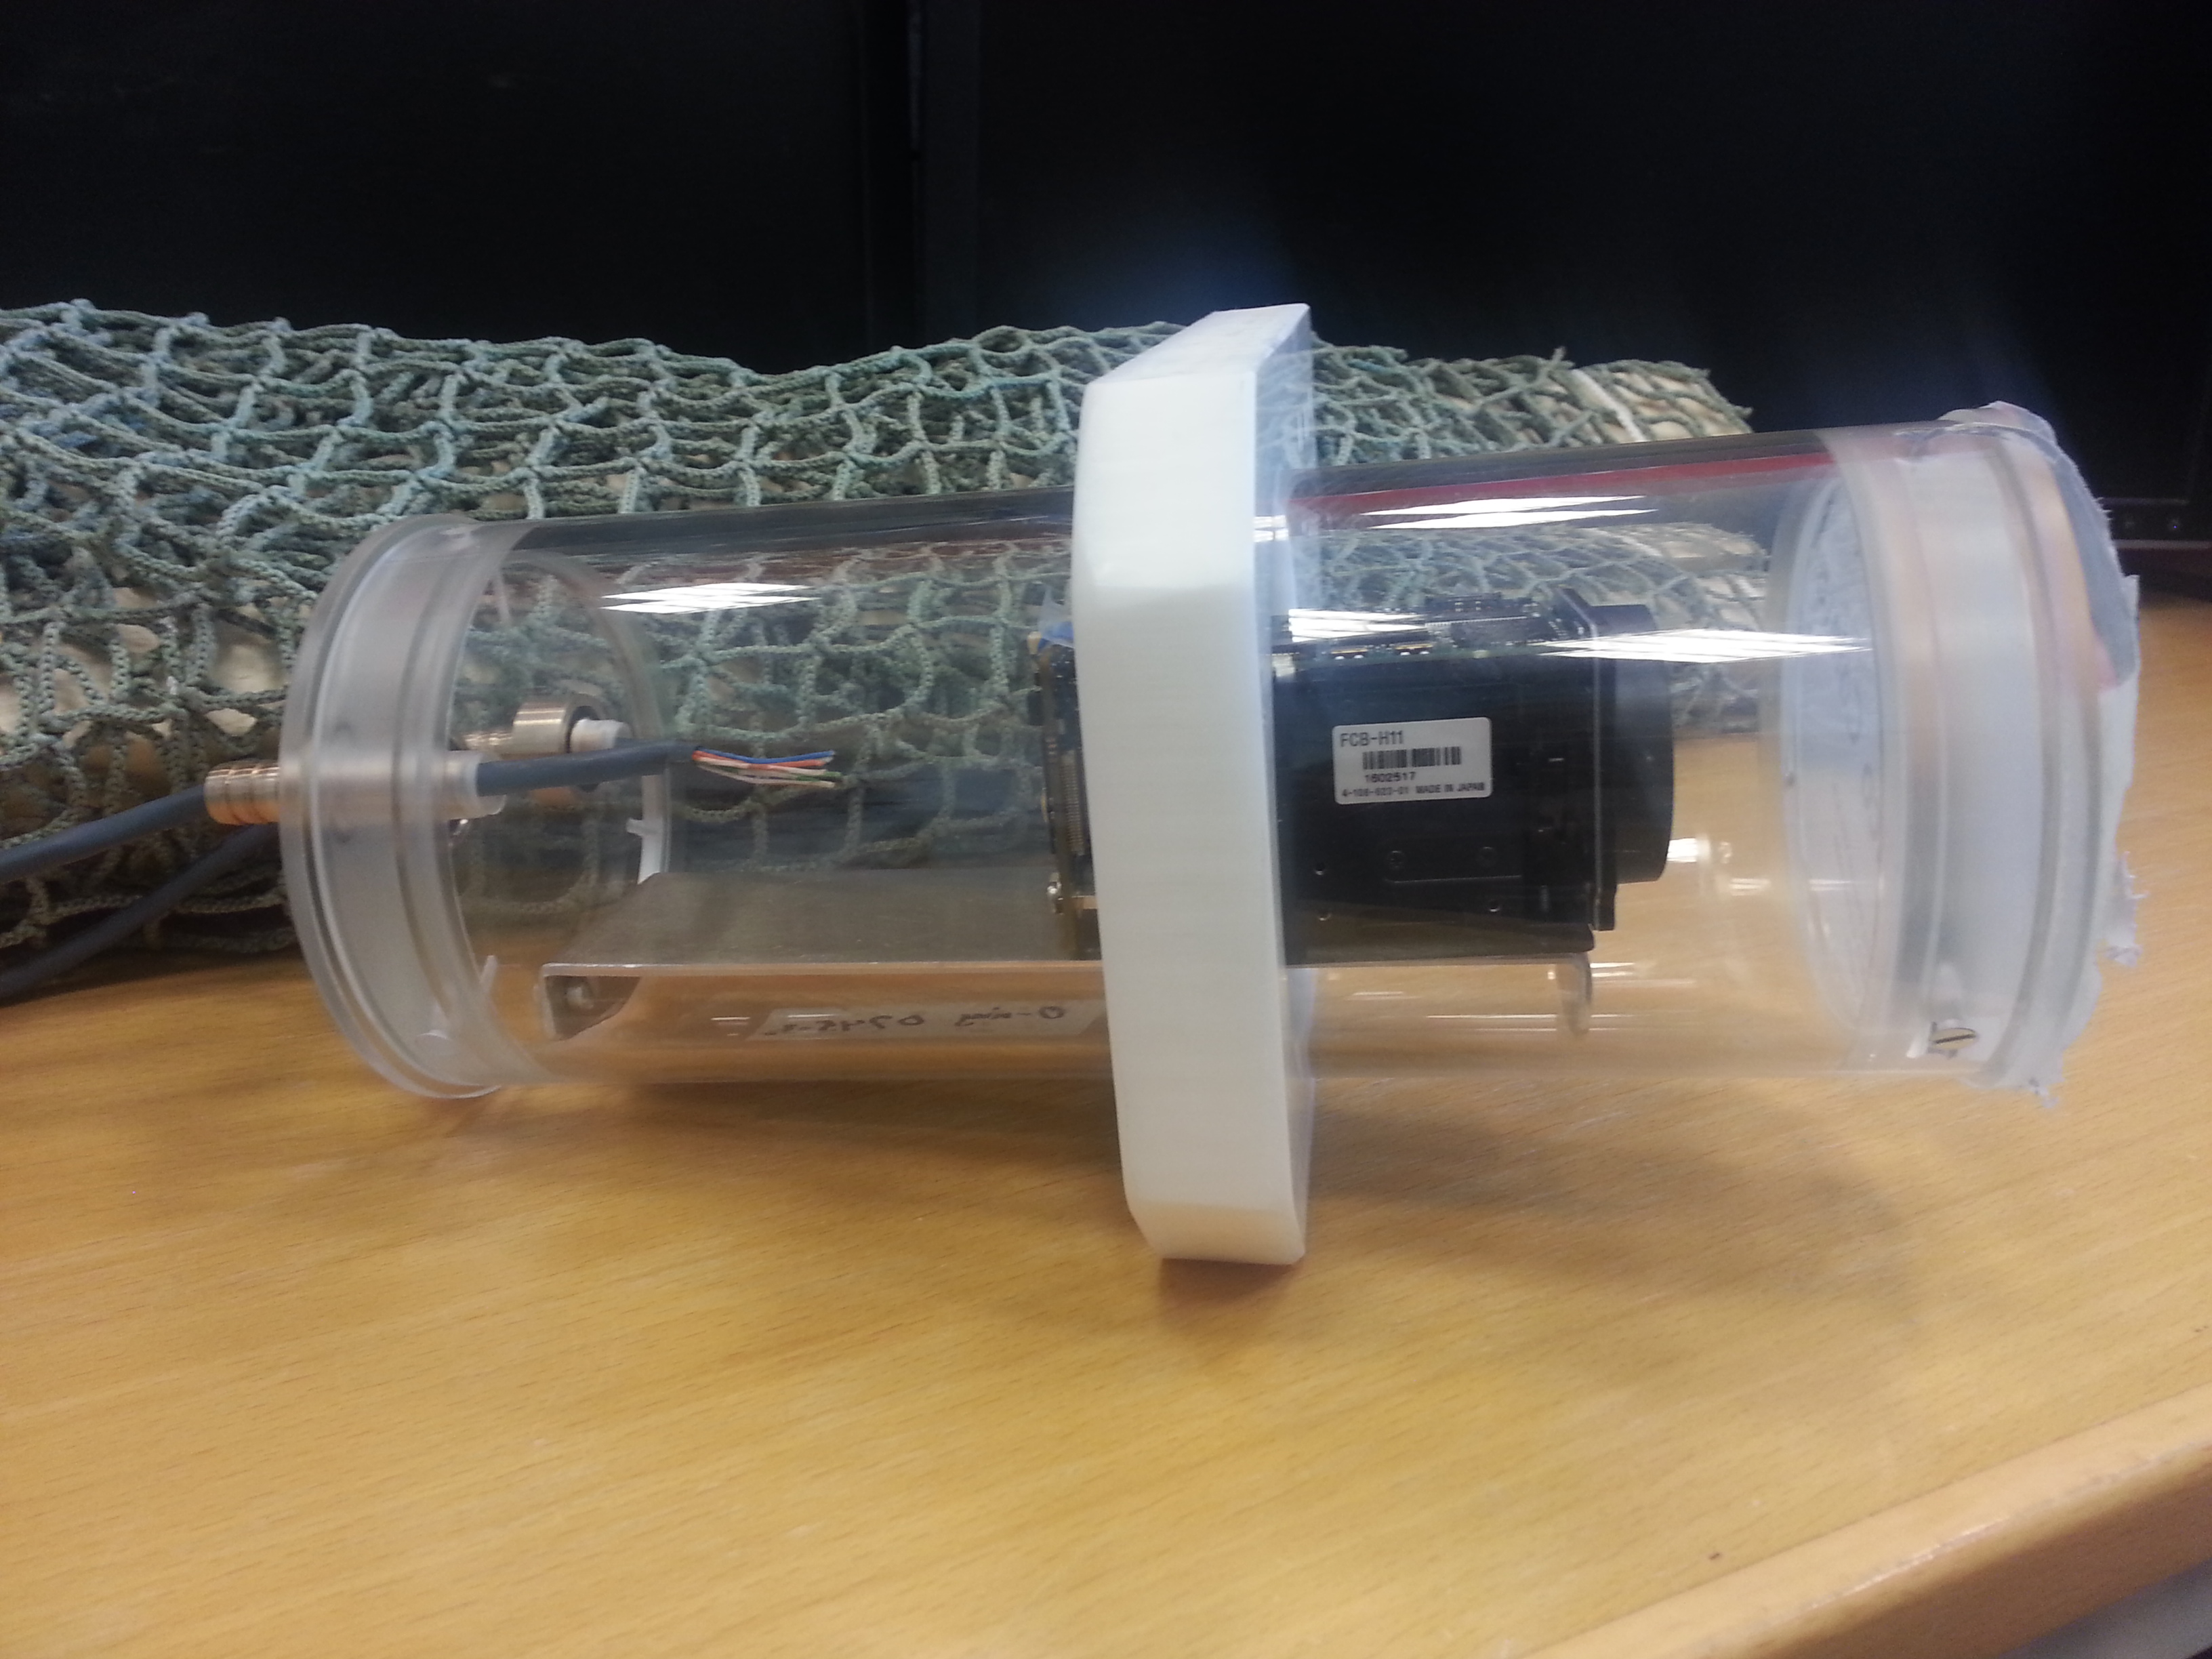
\includegraphics[width=0.94\textwidth]{camera_housing}
 	\caption{Underwater housing designed by the Terje Haugen at the mechanical workshop at the institute with camera seated at the holding bracket. Nipples for the 
 		water tight cable connection using a normal 75 $\Omega$ coaxial cable for the video and a Ethernet CAT-5E twisted pair cable for power and serial data.}
 	\label{fig:housing}
\end{figure}

As seen in figure \ref{fig:housing} the housing also comes with a outer mounting bracket in white acrylic. This is used to attach the housing to the underwater 
part of the rig as described in section \vref{sec:test.rig}. Both the front and back cover of the housing is removable using three screws. To ensure that 
the housing is waterproof there are also a slot on each cover that has a o-ring that gives a tight seal between the inside of the housing and the covers.

\subsection{Underwater Lights}

To mimic the setup from Argus described in \vref{sec:spec.underwater.light}, some cheaper LED based lights were bought. The lights are two casings 
which delivers \SI{27}{\watt}. Each casing has 9 LEDS, each rated to \SI{3}{\watt}. The lights are shown in figure \vref{fig:underwater_light}.

\begin{figure}[htbp]
	\centering
	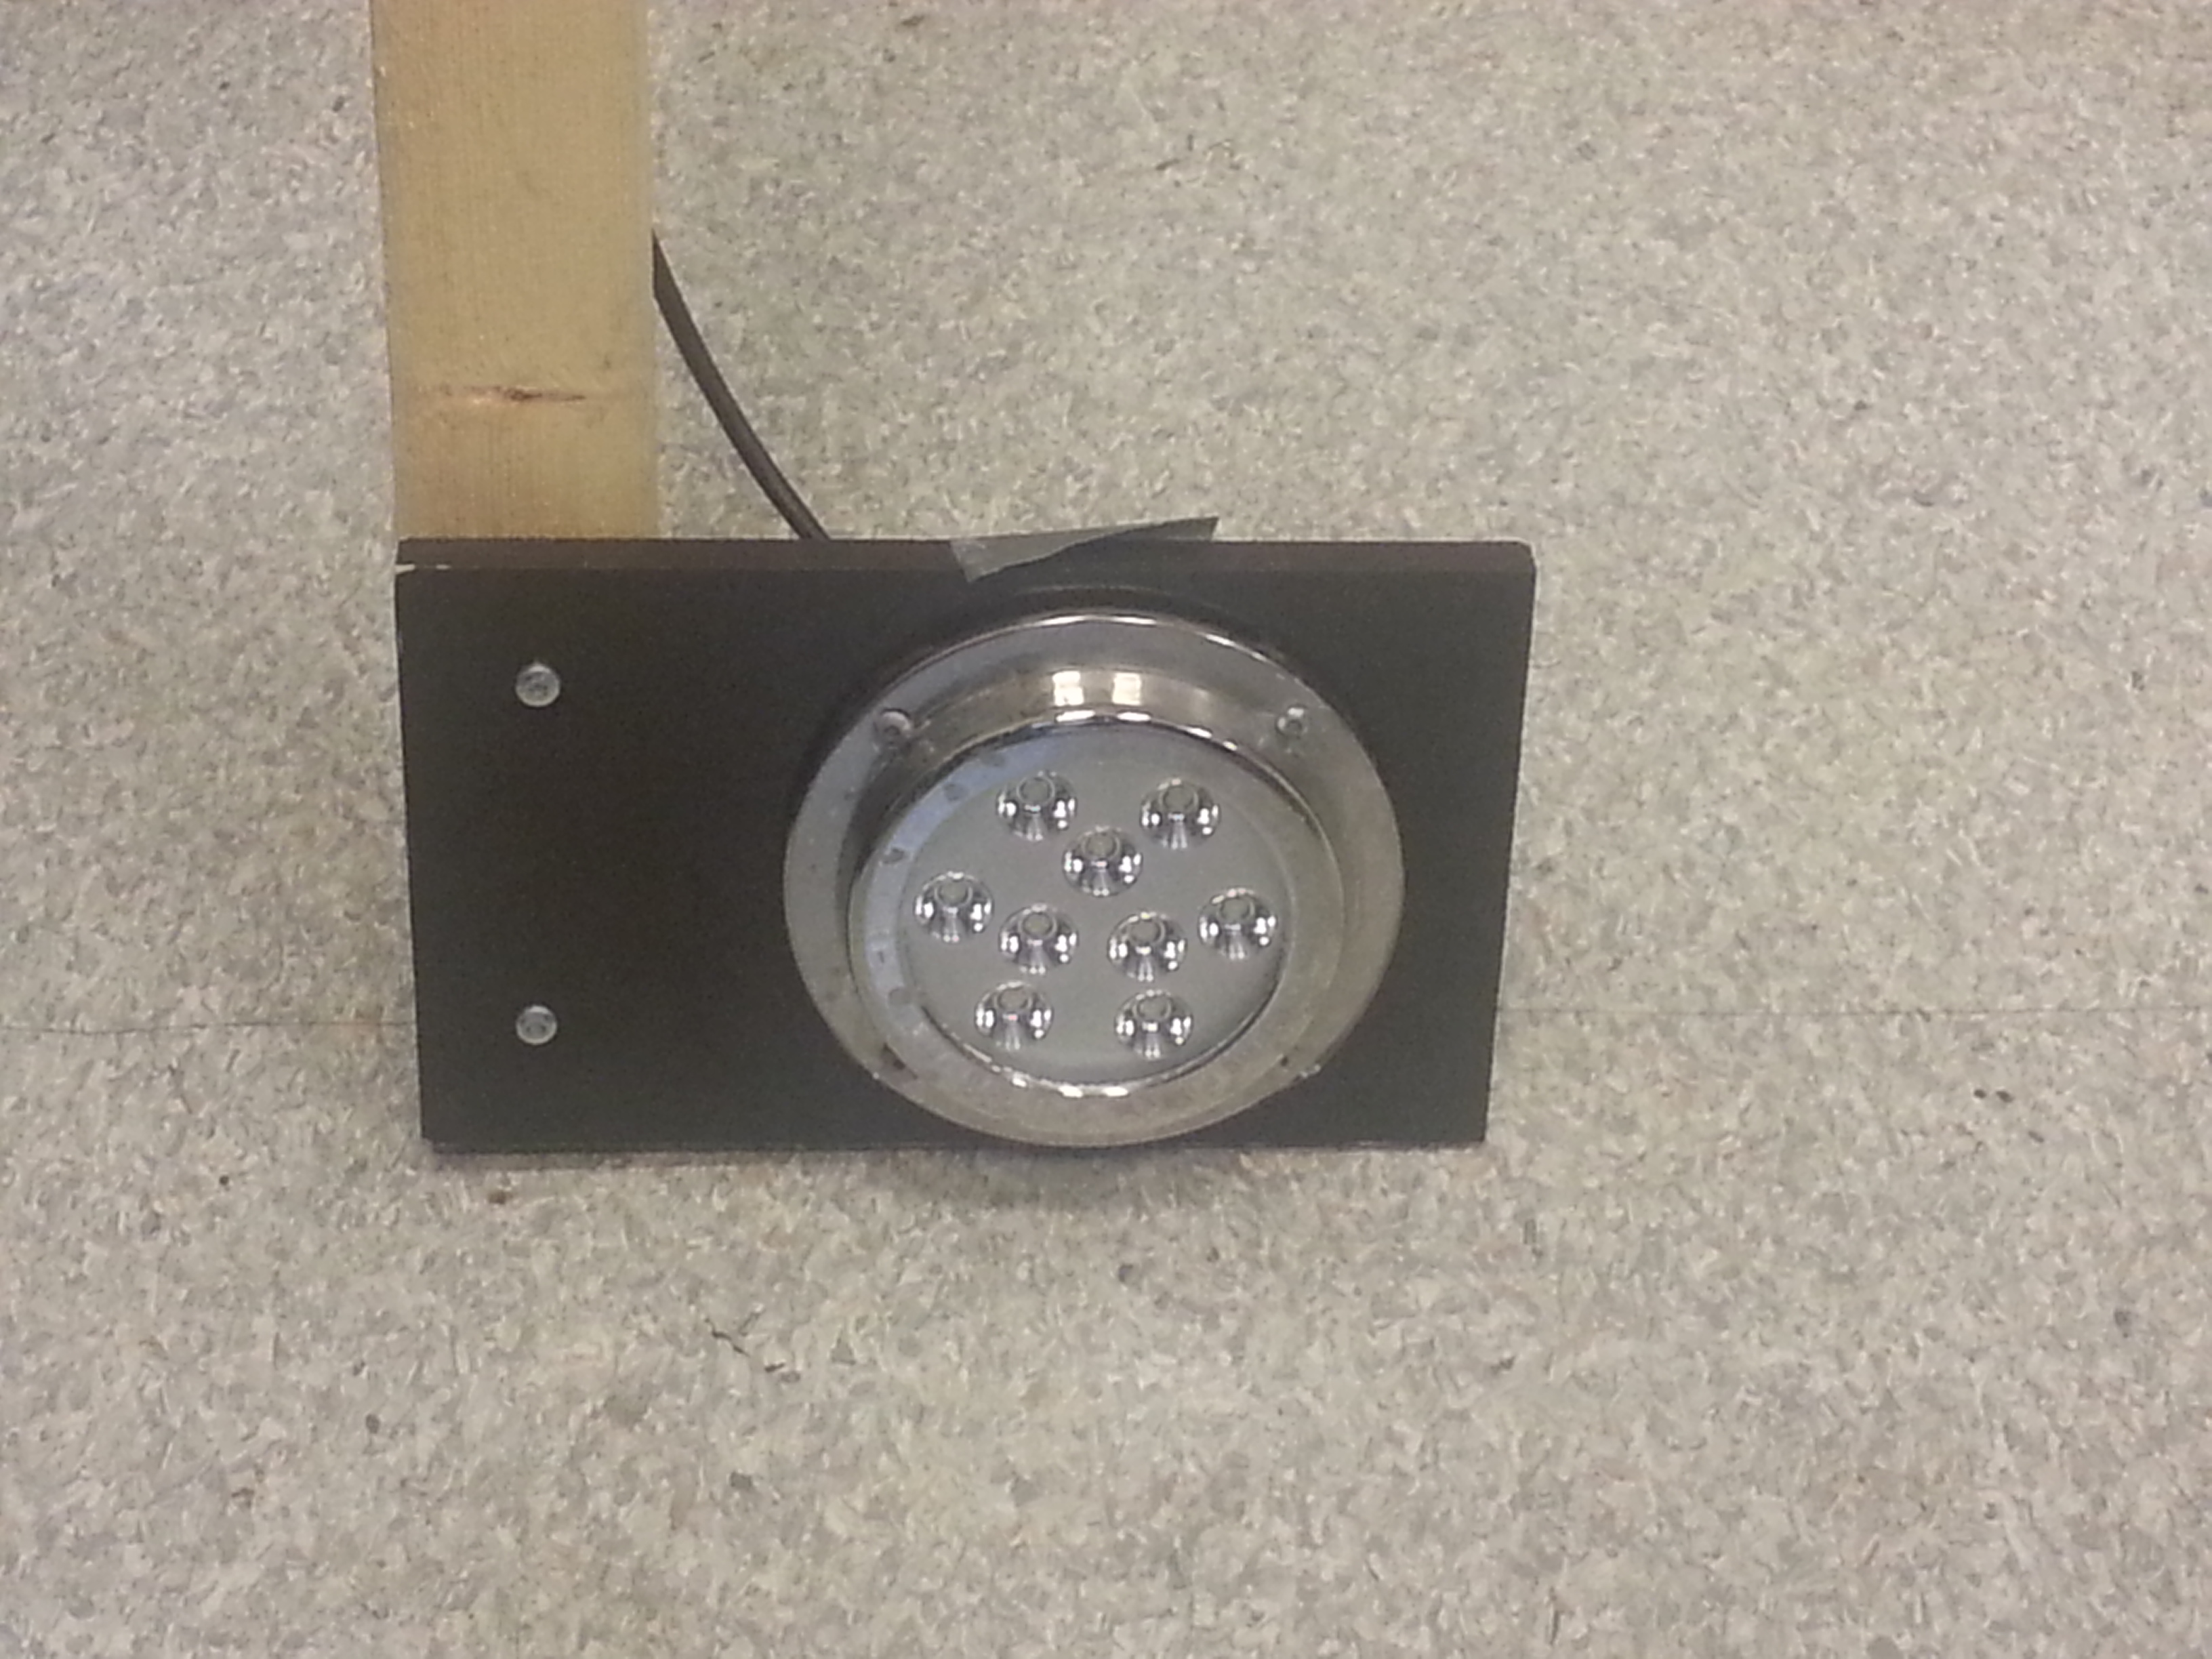
\includegraphics[width=0.8\textwidth]{led_light}
	\caption{Underwater LED lights mounted on a plywood backing plate}
	\label{fig:underwater_light}
\end{figure}

The lights are originally meant to be mounted on a ships hull to light up the surrounding waters of the boat. 
This means that the lights are designed for mounting on top of a flat surface, which makes things easier for us. It 
is also delivered with a \SI{12}{\volt DC} driver which means that it can be connected to any 
\SI{12}{\volt} source.

\subsection{Cabling}
The cabling used 


\subsection{Hardware Schematic}

\begin{sidewaysfigure}
	\centering
	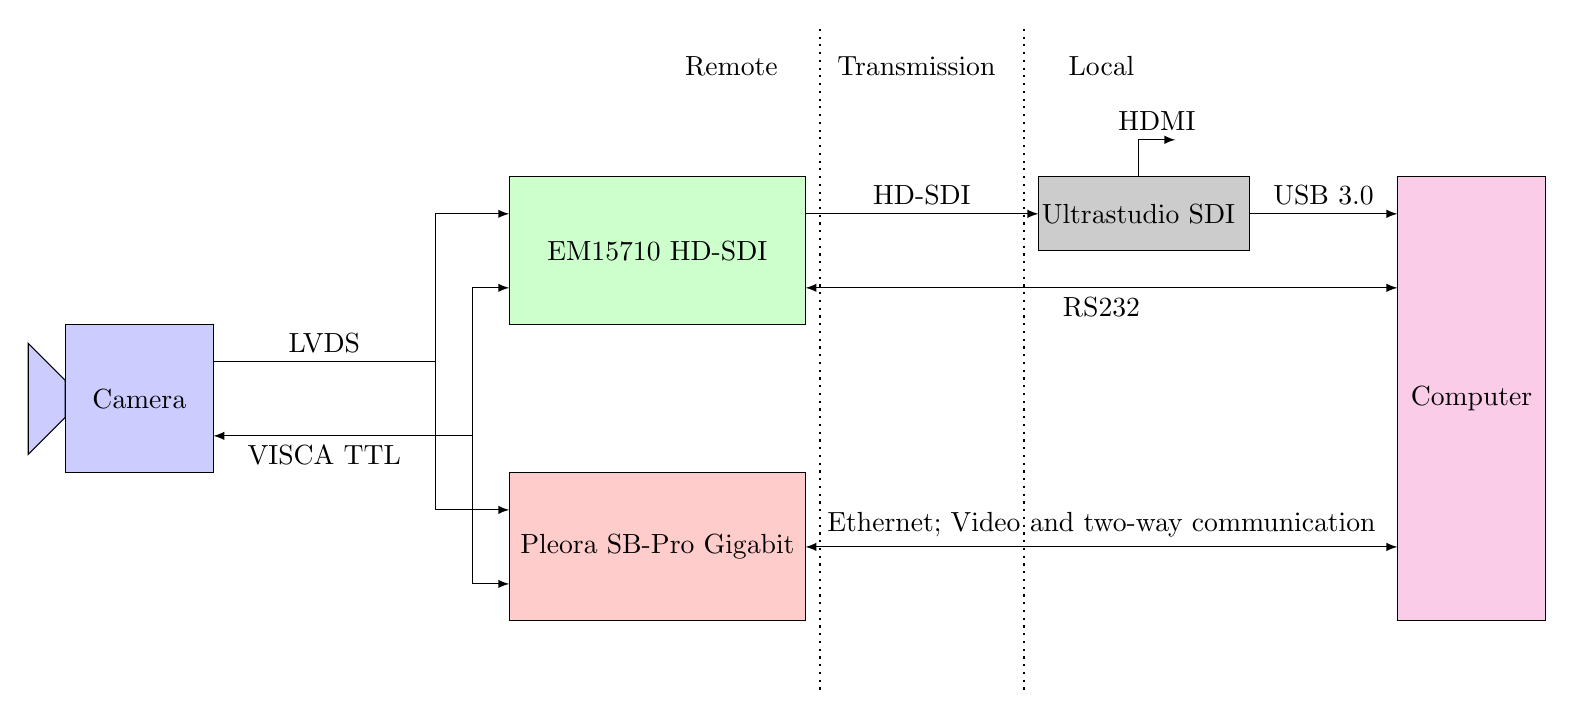
\begin{tikzpicture}[scale=0.94]
		% Camera
		\filldraw[fill=blue!20!white] (0,1) rectangle (2,-1);
		\filldraw[fill=blue!20!white] (0,0.25) -- (-0.5,0.75) -- (-0.5,-0.75) -- (0,-0.25) -- (0,0.25);
		\filldraw[fill=blue!20!white,draw=blue!20!white] (-0.1,-0.25) rectangle (0,.1,0.25);
		\node() at (1,0) {Camera};
		
		% EM
		\filldraw[fill=green!20!white] (6,1) rectangle (10,3);
		\node() at (8, 2) {EM15710 HD-SDI};
		
		% PL
		\filldraw[fill=red!20!white] (6,-1) rectangle (10,-3);
		\node() at (8, -2) {Pleora SB-Pro Gigabit};
		
		% U-SDI
		\filldraw[fill=black!20!white] (13.15,2) rectangle (16,3);
		\node() at (14.5, 2.5) {Ultrastudio SDI};
		
		% PC
		\filldraw[fill=magenta!20!white] (18,-3) rectangle (20,3);
		\node() at (19,0) {Computer};
		
		% Horiz lines
		\draw[thick,dotted] (10.2,5) -- (10.2,-4);
		\draw[thick,dotted] (12.95,5) -- (12.95,-4);
		
		% Top lines
		\node() at (9, 4.5){Remote};
		\node() at (11.5, 4.5){Transmission};
		\node() at (14, 4.5){Local};
		
		% Signal lines from camera
		\draw[] (2, 0.5) -- (5, 0.5) node [midway, above] {LVDS};
		\draw[-latex] (5, -0.5) -- (2, -0.5) node [midway, below] {VISCA TTL};
		
		% Signal lines to EM
		\draw[-latex] (5, 0.5) -- (5, 0.5) -- (5, 2.5) -- (6, 2.5);% LVDS
		\draw[-latex] (5, -0.5) -- (5.5, -0.5) -- (5.5, 1.5) -- (6, 1.5); % TTL
		
		% Signal lines to PL
		\draw[-latex] (5, 0.5) -- (5, 0.5) -- (5, -1.5) -- (6, -1.5); % LVDS
		\draw[-latex] (5, -0.5) -- (5.5, -0.5) -- (5.5, -2.5) -- (6, -2.5); % TTL
		
		% Signal line from EM to U-SDI
		\draw[-latex] (10,2.5) -- (13.15, 2.5) node [midway, above]{HD-SDI};
		
		% Signal line from U-SDI, HDMI
		\draw[-latex] (14.5,3) -- (14.5, 3.5) -- (15, 3.5) node [midway, above]{HDMI};
				
		% Signal line from EM to PC
		\draw[latex-latex] (10,1.5) -- (18, 1.5) node [midway, below]{RS232}; 
		
		% Signal line from U-SDI to PC
		\draw[-latex] (16, 2.5) -- (18, 2.5) node [midway, above]{USB 3.0};
		
		% Signal line from PL to PC
		\draw[latex-latex] (10,-2) -- (18, -2) node [midway, above]{Ethernet; Video and two-way communication}; 
	\end{tikzpicture}
	\caption{Schematics of the hardware, showing both the HD-SDI and the Ethernet pipeline. The different signals and directions are drawn in. 
		Vertical lines express different domains in the system; Remote things on the camera, Transmission for the place where the long distance signals are sent and Local for what is 
		near the computer and the receiving end.}
	\label{fig:hw.schema}
\end{sidewaysfigure}

\subsection{Test Rig}\label{sec:test.rig}

\section{Software}

\subsection{Capture Software}

\subsection{Capture constraints}
\cleardoublepage{}


\chapter{Discussion}

\section{Algorithms}

\subsection{Contour based tracking}


\section{Computational complexity and optimizations}
\todo{!}

\subsection{Pyramids}
\todo{!}

\subsubsection{Mimic peripheral vision}


\subsection{Filtering}
\todo{!}

\subsection{Parallel computation}

\subsection{Hardware accelerated computation}

\subsection{Quantifying bounds of aliasing and velocity}
\cleardoublepage{}


\chapter{Conclusion}

\cleardoublepage{}


\chapter{Further Work}

\cleardoublepage{}

\renewcommand*{\bibname}{References}
\bibliographystyle{plainnat}
\bibliography{bibliography}

%% Uncomment the following if you have any appendix
 \appendix
 \addtocontents{toc}{%
  \protect\vspace{1em}% 
  \protect\noindent \bfseries \appendixtocname\protect\par
  \protect\vspace{-.5em}%
 }
% \renewcommand{\chaptername}{\appendixname}
%% include below possible appendices (chapters)
% !TeX spellcheck = nb_NO

\section{Kondensatorligninger}\label{appendix:cond}
I disse avsnittene er ligningene for parallellplatekondensator, \vref{appendix:parallel}, og 
variabel kapasitanskondensatorer, \vref{appendix:var_cap} gjengitt. 
\subsection{Parallellplatekondensator}\label{appendix:parallel}
Ved å bruke definisjonen av strøm
\begin{equation}
	\frac{\mathrm{d}}{\mathrm{d}t}q(t) = i(t)
	\label{eq:i}
\end{equation}
sammen med ligning \eqref{eq:capactiance} får vi
\begin{equation}
	i(t) = \frac{\mathrm{d}}{\mathrm{d}t}\big(C(t)v(t)\big)
	\label{eq:cap_iv}
\end{equation}

Ligning \eqref{eq:cap_iv} gir en sammenheng mellom strøm gjennom en kondensator og spenning over kondensatoren. 
Det er også tydelig av ligningen at det må legges en varierende spenning 
over kondensatoren for å den skal lede. 

Ved å løse \eqref{eq:cap_iv} med hensyn på \(v(t)\) får vi
\begin{equation}
	v(t) = \frac{1}{C} \int^t_{-\infty}{i(\tau)\,\mathrm{d}\tau}
	\label{eq:cap_v}
\end{equation}
som er standardlikningen for spenningsutvikling over en kondensator ved en variabel strøm, gitt at $C$ er konstant. 

\subsection{Variabel kapasitansligning}\label{appendix:var_cap}
Antagelsen i appendiks \vref{appendix:parallel} er feil, da vi i denne oppgaven 
er ute etter å måle akkurat den \(C\) som varierer med tid, \(C(t)\). 
Om vi bruker definisjonen for \(i(t)\) fra ligning \eqref{eq:i} sammen 
med \eqref{eq:cap_iv}, får vi
\begin{align}
	i(t)  
	&= \frac{\mathrm{d}}{\mathrm{d}t} \big( C(t)v(t) \big)\label{eq:i.3}\\
	&= v(t)\frac{\mathrm{d}}{\mathrm{d}t}C(t) + C(t)\frac{\mathrm{d}}{\mathrm{d}t}v(t) \label{eq:i.4}
\end{align}

Som vi ser av ligning \eqref{eq:i.3} er det umulig å løse dette problemet eksplisitt med tanke på \(C(t)\) 
uten å gjøre antagelse om \(v(t)\) eller \(i(t)\).

Resultatet i ligning \eqref{eq:i.4} er hovedgrunnen til at det ikke er 
mulig å finne absoluttverdier i denne oppgaven.

\section{Enkel oppladningstidmåling}\label{appendix:oppladning}
Som et enkelt eksempel på hvordan er kapasitiv måling kan gjøres, er eksemplet under tatt med. 


En enkel algoritme i pseudokode er også gjengitt. 

\begin{center}
	\begin{circuitikz} \draw
	(0,0) node[anchor=east]{Drivpinne}
		to[short, o-*] (1,0)
		to[R, l=, *-*] (1,2)
	(0,2) node[anchor=east]{Sensorpinne}
		to[short, o-*] (1,2)
		to[C,l=Miljø, *-] (3,2)
		to[short] (3,1) node[ground]{}
	;\end{circuitikz}
\end{center}


%\begin{verbatim}[H]
%\SetAlgoLined
%\KwResult{teller $\propto$ ladetid}
%Initialiser\;
%Set drivpinne høy\;
%\While{sensorpinne ikke høy}{
%	inkrementer teller\;
%}
%\eIf{teller > 0}{
%	resultat = teller\;
%}{
%	feil\;
%}
%\end{verbatim}

Algoritmen over vil gi et tall som er proporsjonalt med antall sykler som er gjort før 
sensorpinnen er kommet opp på logisk 1 ($\approx \frac{V_{dd}}{2}$). Dette er derfor en ''single slope'' måling.

\section{Ladningsoverføring}\label{appendix:mutualcapacitance}
I denne oppgaven er QMatrix\texttrademark fra Atmel valgt som implementasjon av ladningsoverføringsmåling. Atmel utgir dokumentasjon \citet{qtan0079} for de forskjellige teknologiene 
som benyttes og kodebiblioteker for integrasjon i prosjekter.

Den teknologien som er brukt her har sin rot i algoritmen i appendiks \vref{appendix:oppladning}. Det er riktignok en mer komplisert utgave, der hele 
lesesyklusen er vist i appendiks \vref{appendix:mutualcapacitance.4} og i figur \vref{fig:cycle}. En nærmere gjennomgang av 
QMatrix er tilgjengelig i \citet{quantum2006}[QMatrix Technology Whitepaper].

Figur \vref{fig:qmatrix} viser hvordan QMatrix teknologien virker på en pekeflate, som er den primære bruken for QMatrix. 

\begin{figure}[htbp]
	\centering
	\includegraphics[width=0.8\textwidth]{img/qmatrix}
	\caption{QMatrix, hentet fra \citet{quantum2006}}
	\label{fig:qmatrix}
\end{figure}


\clearpage
\subsection{Krets}\label{appendix:mutualcapacitance.circuit}

I figur \vref{fig:chargetransfer} er kretsskjemaet som er brukt i denne oppgaven. Dette skjemaet viser kun 4 punkter, men det er en enkel utvidelse å 
bruke denne kretsen på \(n+m\) punkter som forsøkt vist med subskriptene på linjene.

\begin{figure}[H]
\begin{center}
	\begin{circuitikz}[scale=1.1]
	\draw[dashed,rounded corners] (7.5,9.5) rectangle (5.5,7.5);
	\foreach \x in {8,9} {
		\foreach \y in {6,7} {
			\node[circle,draw] at (\y,\x) {};
		}
	}
	\node[above] at (7.5,9.5) {Membran fra figur \vref{fig:sampl_point}};
	
	\draw
	(0,0) node[anchor=east]{SMP}
		to[short, o-*] (1,0)
		to[R, l=$\text{RYB}_0$] (1,2)
		to[short] (1,3)
		to[short] (0,3)
	(0,3) node[anchor=east]{$\text{YB}_0$}
		to[short, o-*] (1,3)
		to[short] (1,4)
		to[C, l=$\text{CS}_0$] (1,5)
	(0,2) node[anchor=east]{$\text{YB}_m$}
		to[short, o-*] (3,2)
		to[R, l=$\text{RYB}_m$] (3,0)
		to[short] (1,0)
	(3,2) node{}
		to[short] (3,4)
		to[C, l=$\text{CS}_m$] (3,5)
	(0,6) node[anchor=east]{$\text{YA}_m$}
		to[short,o-*] (3,6)
		to[short] (3,5)
	(0,7) node[anchor=east]{$\text{YA}_0$}
		to[short,o-*] (1,7)
		to[short] (1,5)
	(3,6) node{}
		to[R, l=$\text{RY}_m$] (5,6)
		to[short] (7,6)
		to[short] (7,9)
	(1,7) node{} 
		to[short] (3,7)
		to[R, l=$\text{RY}_0$] (5,7)
		to[short] (6,7)
		to[short] (6,9)
	(0,8) node[anchor=east]{$\text{X}_n$}
		to[short, o-*] (3,8)
		to[R, l=$\text{RX}_n$] (5,8)
		to[short] (7,8)
	(0,9) node[anchor=east]{$\text{X}_0$}
			to[short, o-*] (3,9)
			to[R, l=$\text{RX}_0$] (5,9)
			to[short] (7,9)
	;\end{circuitikz}
\end{center}
\caption{Ladningsoverføringskrets}
\label{fig:chargetransfer}
\end{figure}

\pagebreak
Forkortelser og linjer brukt i figur \vref{fig:chargetransfer} er beskrevet under.

\begin{description}
	\item[$\text{X}_n$] Drivlinjene. Kobles til en I/O port.
	\item[$\text{YA}_m$] I/O Porter. Her vil spenningen over $\text{CS}_m$ legge seg. Brukes for å lade ut $\text{CS}_m$.
	\item[$\text{YB}_m$] ADC porter. Måler utviklingen av oppladningen over $\text{CS}_m$.
	\item[SMP] Generel I/O port. Pulser tilbake over $\text{CS}_m$. Dette setter opp en negativ spenning som driver $\text{CS}_m$ tilbake mot 0
	\item[$\text{RYB}_m$] Pull-down resistor 
	\item[$\text{CS}_m$] Samplingkondensator. Lades opp av $\text{X}_m$
\end{description}

Den kretsen som er skissert i figur \vref{fig:chargetransfer} vil ha flere ekvivalenter ettersom hvilken del av oppladningssykelen som kretsen
er i. Disse ekvivalentene er gjennomgått i appendiks \vref{appendix:mutualcapacitance.1}, \vref{appendix:mutualcapacitance.2} og \vref{appendix:mutualcapacitance.3}.

\vfill

\pagebreak
\subsection{Ekvivalenskrets under oppladning}\label{appendix:mutualcapacitance.1}
\begin{figure}[H]
\begin{center}
	\begin{circuitikz}[scale=1.3]
	\draw[dashed,rounded corners] (7.5,9.5) rectangle (5.5,7.5);
		\foreach \x in {8,9} {
			\foreach \y in {6,7} {
				\node[circle,draw] at (\y,\x) {};
			}
		}
		\node[above] at (7.5,9.5) {Membran fra figur \vref{fig:sampl_point}};
		
	
	\draw
	(0,0) node[anchor=east]{SMP}
		to[short, o-*] (1,0)
		to[R, l=$\text{RYB}_0$] (1,2)
		to[short] (1,3)
		to[short] (1,4)
		to[C, l=$\text{CS}_0$] (1,5)
	(0,-1) node[ground]{}
		to[short](0,0)
	%(0,3) node[anchor=east]{$\text{YB}_0$}
	%	to[short, o-*] (1,3)
	%	to[short] (1,4)
	%	to[C, l=$\text{CS}_0$] (1,5)
	%(0,2) node[anchor=east]{$\text{YB}_m$}
	%	to[short, o-*] (3,2)
	%	to[R, l=$\text{RYB}_m$] (3,0)
	%	to[short] (1,0)
	(3,2) node{}
		to[R, l=$\text{RYB}_m$] (3,0)
		to[short] (1,0)
	(3,2) node{}
		to[short] (3,4)
		to[C, l=$\text{CS}_m$] (3,5)
	%(0,6) node[anchor=east]{$\text{YA}_m$}
	%	to[short,o-*] (3,6)
	%	to[short] (3,5)
	%(0,7) node[anchor=east]{$\text{YA}_0$}
	%	to[short,o-*] (1,7)
	%	to[short] (1,5)
	(3,6) node{} 
		to[short] (3,5)
	(1,7) node{}
		to[short] (1,5)
		
	(3,6) node{}
		to[R, l=$\text{RY}_m$] (5,6)
		to[short] (7,6)
		to[short] (7,9)
	(1,7) node{} 
		to[short] (3,7)
		to[R, l=$\text{RY}_0$] (5,7)
		to[short] (6,7)
		to[short] (6,9)
	(0,8) node[anchor=east]{$\text{X}_n$}
		to[short, o-*] (3,8)
		to[R, l=$\text{RX}_n$] (5,8)
		to[short] (7,8)
	(0,9) node[anchor=east]{$\text{X}_0$}
			to[short, o-*] (3,9)
			to[R, l=$\text{RX}_0$] (5,9)
			to[short] (7,9)
	;\end{circuitikz}
\end{center}
\caption{Ekvivalenskrets under oppladning}
\label{fig:chargetransfer_in}
\end{figure}

\pagebreak
\subsection{Ekvivalenskrets under motladning}\label{appendix:mutualcapacitance.2}
\begin{figure}[H]
\begin{center}
	\begin{circuitikz}[scale=1.8] \draw
	(0,5.5) node[ground]{}
		to[short] (0,6)
		to[short] (0,7)
	(0,0) node[anchor=east]{SMP}
		to[short, o-*] (1,0)
		to[R, l=$\text{RYB}_0$] (1,2)
		to[short] (1,3)
		to[short] (1,4)
		to[C, l=$\text{CS}_0$] (1,5)
	(0,3) node[anchor=east]{$\text{YB}_0$}
		to[short, o-*] (1,3)
		to[short] (1,4)
	(0,2) node[anchor=east]{$\text{YB}_m$}
		to[short, o-*] (3,2) 
	(3,2) node{}
		to[R, l=$\text{RYB}_m$] (3,0)
		to[short] (1,0)
	(3,2) node{}
		to[short] (3,4)
		to[C, l=$\text{CS}_m$] (3,5)
	(0,6) node[anchor=east]{$\text{YA}_m$}
		to[buffer] (3,6)
		to[short] (3,5)
	(0,7) node[anchor=east]{$\text{YA}_0$}
		to[short,o-*] (1,7)
		to[short] (1,5)
	(3,6) node{} 
		to[short] (3,5)
	(1,7) node{}
		to[short] (1,5)
		
	%(3,6) node{}
	%	to[R, l=$\text{RY}_m$] (5,6)
	%	to[short] (7,6)
	%	to[short] (7,9)
	%(1,7) node{} 
	%	to[short] (3,7)
	%	to[R, l=$\text{RY}_0$] (5,7)
	%	to[short] (6,7)
	%	to[short] (6,9)
	%(0,8) node[anchor=east]{$\text{X}_n$}
	%	to[short, o-*] (3,8)
	%	to[R, l=$\text{RX}_n$] (5,8)
	%	to[short] (7,8)
	%(0,9) node[anchor=east]{$\text{X}_0$}
	%		to[short, o-*] (3,9)
	%		to[R, l=$\text{RX}_0$] (5,9)
	%		to[short] (7,9)
	;\end{circuitikz}
\end{center}
\caption{Ekvivalenskrets under motladning}
\label{fig:chargetransfer_out}
\end{figure}



\pagebreak
\subsection{Ekvivalenskrets under utladning}\label{appendix:mutualcapacitance.3}
\begin{figure}[H]
\begin{center}
	\begin{circuitikz}[scale=1.5] \draw
	(0,5.5) node[ground]{}
		to[short] (0,6)
		to[short] (0,7)
	(0,0) node[anchor=east]{SMP}
		to[short, o-*] (1,0)
		to[R, l=$\text{RYB}_0$] (1,2)
		to[short] (1,3)
		to[short] (1,4)
		to[C, l=$\text{CS}_0$] (1,5)
	(0,3) node[anchor=east]{$\text{YB}_0$}
		to[short, o-*] (1,3)
		to[short] (1,4)
	(0,2) node[anchor=east]{$\text{YB}_m$}
		to[short, o-*] (3,2) 
	(3,2) node{}
		to[R, l=$\text{RYB}_m$] (3,0)
		to[short] (1,0)
	(3,2) node{}
		to[short] (3,4)
		to[C, l=$\text{CS}_m$] (3,5)
	(0,6) node[anchor=east]{$\text{YA}_m$}
		to[buffer] (3,6)
		to[short] (3,5)
	(0,7) node[anchor=east]{$\text{YA}_0$}
		to[short,o-*] (1,7)
		to[short] (1,5)
	(3,6) node{} 
		to[short] (3,5)
	(1,7) node{}
		to[short] (1,5)
	(0,-1) node[ground]{}
		to[short](0,0)
	%(3,6) node{}
	%	to[R, l=$\text{RY}_m$] (5,6)
	%	to[short] (7,6)
	%	to[short] (7,9)
	%(1,7) node{} 
	%	to[short] (3,7)
	%	to[R, l=$\text{RY}_0$] (5,7)
	%	to[short] (6,7)
	%	to[short] (6,9)
	%(0,8) node[anchor=east]{$\text{X}_n$}
	%	to[short, o-*] (3,8)
	%	to[R, l=$\text{RX}_n$] (5,8)
	%	to[short] (7,8)
	%(0,9) node[anchor=east]{$\text{X}_0$}
	%		to[short, o-*] (3,9)
	%		to[R, l=$\text{RX}_0$] (5,9)
	%		to[short] (7,9)
	;\end{circuitikz}
\end{center}
\caption{Ekvivalenskrets under utladning}
\label{fig:chargetransfer_reset}
\end{figure}

\pagebreak
\section{Ladesykel over \texorpdfstring{$\text{CS}_m$}{Cs}}\label{appendix:mutualcapacitance.4}


\begin{sidewaysfigure}
\begin{figure}[H]
\begin{center}
\begin{tikzpicture}[xscale=15]
	%\draw[help lines,step=0.1] (0,-8) grid (1,7);
	\draw [->, help lines] (0,-7) -- (0,6);
	\draw [->, help lines] (0,0) -- (1,0);
	\draw[rounded corners] (0,0) -- (0.04,1) -- (0.08,1) -- (0.12,2) -- (0.16,2) -- (0.20,3) -- (0.24,3) -- (0.28,4) -- (0.32,4) -- (0.36,5) -- (0.4,5) -- (0.44,4) -- (0.48,4) -- (0.52,3) -- (0.56,3) -- 
		(0.6,2) -- (0.64,2) -- (0.68,1) -- (0.72,1) -- (0.76,0) -- (0.80,0) -- (0.84,-1) -- (0.88,-1) -- (0.92,-2) -- (0.96,-2) -- (1,0);
	\draw[thin,dashed] (0.38,-7) -- (0.38,6);
	\node[above] at (0.36,6) {1. fase ferdig};
	\node[right] at (0.4,5) {Start utladning};
	\draw[thin,dashed] (0.78,-7) -- (0.78,6);
	\node[above] at (0.76,6) {2. fase ferdig};
	\draw[thin,dashed] (0.94,-7) -- (0.94,6);
	\node[above,align=center] at (0.94,6) {3. fase ferdig};
	
	\node[left] at (0,0) {$V_{\text{CS}_m}$};
	\node[left] at (0,-3) {$\text{X}_n$};
	\node[left] at (0,-5) {SMP};
	\node[left] at (0,-7) {$\text{YA}_m$};
	
	\draw[<->] (0.15,3) -- (0.15,4);
	\draw[dashed] (0.2,3) -- (0.15,3);
	\draw[dashed] (0.29,4) -- (0.15,4);
	\node[left] at (0.15,3.5) {$v_\delta$};
	
	\draw[<->]  (0.52,-2.5) -- (0.56,-2.5);
	\draw[dashed] (0.52,-4) -- (0.52,-2.5);
	\draw[dashed] (0.56,-4) -- (0.56,-2.5);
	\node[above] at (0.54,-2.5) {ADC};
	
	\draw [->, help lines] (0,-3) -- (1,-3);
	\draw (0,-2) -- (0.04,-2) -- (0.04,-3) -- (0.08,-3) -- (0.08,-2) -- (0.12,-2) -- (0.12,-3) -- (0.16,-3) -- (0.16,-2) -- (0.2,-2) -- (0.2,-3) -- (0.24,-3) -- (0.24,-2) -- (0.28,-2) -- (0.28,-3) -- 
		(0.32,-3) -- (0.32,-2) -- (0.36,-2) -- (0.36,-3);
	
	\draw [->, help lines] (0,-5) -- (1,-5);
	\draw (0.4,-5) -- (0.4,-4) -- (0.44,-4) -- (0.44,-5) -- (0.48,-5) -- (0.48,-4) -- (0.52,-4) -- (0.52,-5) -- (0.56,-5) -- (0.56,-4) -- (0.60,-4) -- (0.60,-5) -- (0.64,-5) -- (0.64,-4) -- (0.68,-4) -- 
		(0.68,-5) -- (0.72,-5) -- (0.72, -4) -- (0.76,-4) -- (0.76,-5) -- (0.80,-5) -- (0.80,-4) -- (0.84,-4) -- (0.84,-5) -- (0.88,-5) -- (0.88,-4) -- (0.92,-4) -- (0.92,-5);
		
	\draw [->, help lines] (0,-7) -- (1,-7);
\end{tikzpicture}
\end{center}
\caption{Skjematisk tegning av ladesykel over $\text{CS}_m$}
\label{fig:cycle}
\end{figure}
\end{sidewaysfigure}

Figur \vref{fig:cycle} gjengir en full lesesyklus for oppsettet. 

\subsection{Fase 1}
I den første delen av figur \vref{fig:cycle} fungerer kretsen som vist i figur \vref{fig:chargetransfer_in} i appendiks \vref{appendix:mutualcapacitance.1}.

Her blir \(\text{X}_n\) brukt til å øke spenningen over \(\text{CS}_m\). Avhengig av avstanden mellom elektrodene så vil \(v_\delta\) bli større eller mindre, og 
vil dermed endre høyden på pyramiden, da det er et fast antall pulser på \(\text{X}_n\) i denne delen.

\subsection{Fase 2}\label{appendix:down}
I den andre delen av figur \vref{fig:cycle} fungerer kretsen som vist i figur \vref{fig:chargetransfer_out} i appendiks \vref{appendix:mutualcapacitance.2}. 

Her blir porten merket SMP  brukt til å lade alle kondensatorene ut. Mellom hver puls på SMP brukes ADC funksjonaliteten i mikrokontrolleren til å 
måle spenningen som ligger over alle kondensatorene. Om denne går under nullpotensialet vil antall pulser som er brukt i denne delen være et mål 
på hvor mye spenning som ble lagt over kondensatoren. Dette er en klassisk dobbelthelningsmåling\footnote{dual-slope}, som brukes da målingene blir mindre støyutsatt, og 
fysiske endringer med kondensatorene kan motvirkes til en viss grad.

\subsection{Fase 3}
I den tredje delen av figur \vref{fig:cycle} fungerer kretsen som vist i figur \vref{fig:chargetransfer_reset} i appendiks \vref{appendix:mutualcapacitance.3}.

Etter nedladningsdelen i \vref{appendix:down} vil mest sannsynlig flere av kondensatorene ha en negativ spenning, og de må derfor settes tilbake 
til et kjent nullpotensiale slik at oppladningssyklusen begynner fra et kjent spenning.


\end{document} 
